\chapter*{Samenvatting}
\selectlanguage{dutch}

Er is een vakgebied binnen de moderne fysica dat de fundamentele vragen der materie probeert te beantwoorden.
Deze vragen, welke filosofen van alle tijden hebben beziggehouden, gaan over het identificeren en begrijpen
van de fundamentele ondeelbaar bouwstenen waaruit de wereld is opgebouwd. Opmerkelijk is dat meer dan twee
millennia nadat de filosoof Democitus de notie van atomen of \textgreek{άτομα} - Grieks voor ondeelbaar -  heeft ge\"introduceerd,
hedendaagse wetenschappers nog steeds geen sluitende antwoorden hebben op deze fundamentele vragen. Het lijkt erop dat het
zichtbare heelal bestaat een handvol elementaire deeltjes die zijn ondergebracht in twee verschillende categori\"en. Namelijk
{\it gauge bosons}, welke verantwoordelijk zijn voor het medi\"eren van alle bekende krachten tussen de deeltjes
(met de uitzondering van de zwaartekracht), en {\it fermions} welke de bouwblokken zijn van materie. Het recentelijk ontdekte
Higgs deeltje \cite{higgs-cms,higgs-atlas} is een speciaal type boson dat een centrale rol speelt in het genereren van massa
voor deeltjes. Fermions kunnen verder worden onderverdeeld in twee categori\"en. {\it Quarks} vormen samengestelde deeltjes
zoals het proton en het neutron. Het zwaarste quark echter, het \tquark quark, zal vervallen voordat het een samengesteld
deeltje kan vormen. Het bekendste {\it lepton} is het electron. Samen met de protonen en neutronen vormen elektronen de atomen.
Leptonen en quarks spelen een cruciale rol in processen zoals de formatie van sterren en hebben zo een directe impact op de
manier waarop leven op aarde is ge\"evolueerd.

\subsubsection{Deeltjes fysica en Het Standaard Model}
Het Standaard Model is een state of the art mathematisch model dat de interacties tussen fermionen
beschrijft \cite{sm-glashow,sm-weinberg,sm-salam}. Dit is een quantum mechanisch proces.
Het beschrijven zo'n process vereist het berekenen van de kans op een bepaalde uitkomst van het proces.
Dit behelst niet-triviale berekeningen. Het voorspellend vermogen van het Standaard Model kan daarom
worden beschouwd als een belangrijke prestatie. Het recentelijk ontdekte Higgs boson \cite{higgs-cms,higgs-atlas},
dat een belangrijke rol speelt in de verklaring hoe deeltjes massa verkrijgen, maak het Standaard Model compleet.

Ondanks het succes van het Standaard Model, zijn er nog steeds fenomenen en observaties welke het model niet kan verklaren.
Wellicht de meest opvallende is de afwezigheid van een beschrijving van de meest bekende, en toch de meest zwakke, natuurkracht:
de zwaartekracht. Een ander voorbeeld betreft antimaterie; een toestand van materie, waarbij de quantum numbers voor elektrische
lading en pariteit omgekeerd zijn aan die van materie. De waargenomen materie-antimaterie disbalans in het
heelal \cite{more-cpv-huet,more-cpv-gavela_I,more-cpv-gavela_II} is niet voldoende beschreven in het Standaard Model.
De bovenstaande fenomenen zijn slechts een paar voorbeelden die de onvolledigheid van het model blootleggen.
Daarom is het des te meer van belang de voorspellingen van het Standaard Model wetenschappelijk te toesten en zo het model te
verbeteren. Significante verschillen tussen de metingen en de voorspellingen kunnen een aanwijzing zijn voor {\it Nieuwe Fysica}.

\subsubsection{\CP schending en Nieuwe Fysica}
Materie en antimaterie zijn gecre\"eerd in gelijke hoeveelheden tijdens de eerste fase van de oerknal, aldus de
gevestigde theori\"en \cite{more-cpv-huet,more-cpv-gavela_I,more-cpv-gavela_II}. Dit idee suggereert de notie van
een symmetrie tussen materie en antimaterie: \CP symmetrie. Perfecte \CP symmetrie betekent dat interacties van
materie op dezelfde manier verlopen als interacties van antimaterie. Echter, het huidige heelal bestaat bijna
geheel uit materie. Het ontstaan van  {\it \CP schending} is een vraagstuk waar het Standaard Model geen
sluitende verklaring voor geeft.

Het idee dat de natuur processen prefereert waar de betrokken deeltjes materie zijn boven processen waar de
deeltjes antimaterie zijn wordt beschreven in het Standaard Model. Echter, het model kan de grootte van de
asymmetrie tussen materie en antimaterie niet voldoende verklaren. Daarom wordt er gezocht naar andere bronnen
van \CP schending, buiten het Standard Model. Een manier om hier naar te zoeken is door  die parameters te
bestuderen waar de Standaard Model een minimale \CP schending voorspelt. Een significante observatie van \CP
schending geeft dan een directe hint voor de aanwezigheid van Nieuwe Fysica. Het verzamelen van veel van zulke
hints helpt fysici bij het identificeren van de zwakke plekken in het Standaard Model. Daarnaast geeft het
richting aan de zoektocht naar alternatieve modellen, zoals {\it Supersymmetry}  \eg \cite{Golfand:1971iw,Volkov:1973ix,Wess:1974tw}.

\begin{figure}[t]
  \begin{subfigure}{0.5\textwidth}
    \raggedright
    {\scalebox{1}{\sffamily \input{Figures/Chapter1/tree}}}
    \caption{}
    \label{app_nl_jpsiphi_tree}
  \end{subfigure}%
  \hfill
  \begin{subfigure}{0.5\textwidth}
    \raggedleft
    {\scalebox{1}{\sffamily %%BoundingBox: -5 0 121 170
%%HiResBoundingBox: -5 0 120.57008 169.36447

\begin{fmffile}{Figures/Chapter1/penguin}
  \fmfframe(17,-25)(31,-25){
    \begin{fmfgraph*}(115,170)
      \fmfstraight
      \fmfleft{i0,i1,i2,i3,i4,i5}
      \fmfright{o0,o1,o2,o3,o4,o5}
      \fmf{fermion,tension=1.8,label.side=left,label=b}{v5,i3}
      \fmf{fermion,tension=1.5,right=0.2,label.side=left,label={\hspace*{18pt}u,,c,,t}}{v2,v5}
      \fmf{gluon,tension=2}{v4,v2}
      \fmf{dbl_dashes,tension=0}{v4,v2}
      \fmf{fermion,tension=0.3,right=0.2,label.side=left }{v3,v2}
      \fmf{boson,tension=0.6,left=0.3,label=W$^+$,label.side=left}{v3,v5}
      \fmf{fermion,label=c,tension=0.9,right=0.3,label.side=left}{o4,v4}
      \fmf{fermion,label=c,tension=0.9,right=0.3,label.side=left}{v4,o3}
      \fmf{fermion,label=s,label.side=left}{o2,v3}
      \fmffreeze
      \fmf{fermion,tension=0.7,label=s,label.side=left}{v1,o1}
      \fmf{fermion,tension=1,label.side=left,label=s}{i2,v1}
      %\fmf{phantom,tension=0.4}{v4,v1}
      \fmf{phantom,tension=0.4}{v3,v1,v5}
      \fmf{plain,right=0.2}{i2,i3}
      \fmf{plain,left=0.2,label=$\Bs$}{i2,i3}
      \fmf{plain,right=0.2,label=$\phi$}{o1,o2}
      \fmf{plain,left=0.2}{o1,o2}
      \fmf{plain,right=0.2,label=$\jpsi$}{o3,o4}
      \fmf{plain,left=0.2}{o3,o4}
    \end{fmfgraph*}
  }
\end{fmffile}
}}
    \caption{}
    \label{app_nl_jpsiphi_peng}
  \end{subfigure}
     \caption{Eerste orde {\it tree} (links) en hogere order {\it pingu\"in} (rechts) \BsJpsiPhi verval diagrammen.}
  \label{app_nl_jpsiphi_tree_peng}
\end{figure}

\subsubsection{De zwakke fase \phis}
Een interessante parameter waar de Standaard Model een waarde van ongeveer nul voorspelt is de zwakke fase \phis.
Deze parameter manifesteert zichzelf in de interactie $\bquark\to\cquark\cquarkbar\squark$, waar een \bquark
vervalt naar drie andere quarks. Een veelbelovend vervalkanaal voor de meting van \phis is \BsJpsiPhi,
zie \figref{app_nl_jpsiphi_tree}. De Standaard Model voorspelling van \phis en de meest precieze meting van deze
parameter door \lhcb zijn:

\begin{subequations}
  \label{app_nl_phis_lhcb_theo}
  \begin{align}
  \centering
  \phiS{\lhcb}           &=  -0.010 \pm 0.039  \quad {\rm rad},
  \label{app_nl_phis_lhcb}\\
  \phiS{SM,tree}  &= -0.03761 \; ^{+0.00073}_{-0.00082}  \quad {\rm rad}.
  \label{app_nl_phis_theo}
\end{align}
\end{subequations}


\noindent Uit bovenstaande meting volgt dat de waarde van \phis is overeenstemming is met de Standaard Model voorspelling.
Elke mogelijke bijdrage van Nieuwe Fysica aan \phis moet daarom heel klein zijn. Vanuit het experimentele oogpunt wordt
deze meting nu pas echt interessant: de statistische onzekerheid van de meting is bijna klein genoeg om een verschil tussen
de gemeten waarde en de SM voorspelling aan te kunnen tonen. De toekomstige metingen van \phis markeren dan ook een tijdperk
van hoge precisie metingen, waar het bestaan van Nieuwe Fysica al dan niet zal worden aangetoond.

Echter, wanneer experimentele metingen met zulke hoge precisie kunnen worden uitgevoerd
kunnen zelfs de kleinste effecten zichtbaar worden. Er is een belangrijke bijdrage aan de
experimentele meting van \phis welke tot dusver niet in acht werd genomen. Het betreft de
bijdragen van zogenaamde {\it pingu\"in topologi\"en}, zie  \figref{app_nl_jpsiphi_tree_peng}.
Hoewel de bijdragen van deze pingu\"in topologi\"en klein zijn, zullen ze de Standaard Model
voorspelling, $\phis^{\tiny \text{SM,tree}}$, veranderen met $\Delta\phiS{peng}$. Gegeven het
feit dat potenti\"ele Nieuwe Fysica bijdragen aan $\phis$ klein zijn (\equref{app_nl_phis_lhcb_theo}),
is het van cruciaal belang de bijdragen van pinguin topologi\"en te onderscheiden van die door Nieuwe Fysica.
Immers, Nieuwe Fysica verandert de Standaard Model voorspelling ook met een kleine waarde
 $\Delta\phis^{\tiny \text{NP}}$, zoals weergegeven in de volgende vergelijking:

\begin{equation}
\centering
 \phis^{\text {eff}} = \phis^{\tiny \text{SM,tree}} + \Delta\phiS{peng} + \Delta\phis^{\tiny \text{NP}},
 \label{app_nl_phis_sm_peng}
\end{equation}

\noindent met $\phis^{\text {eff}}$ de experimentele \phis meting. Het is dus van groot belang de
bijdragen van pingu\"in topologi\"en correct af te schatten. Hiervoor worden andere \Bs vervalkanalen gebruikt,
zogenaamde controle kanalen. De gekozen controle kanalen, bijvoorbeeld \BsJpsiKst hebben dezelfde tree en
pingu\"in topologi\"en als \BsJpsiPhi. Door gebruik te maken van bepaalde quark symmetri\"en is het
mogelijk om nauwkeurig de grootte van $\Delta\phiS{peng}$ te bepalen. Dit is noodzakelijk voor precieze
meting van $\Delta\phis^{\tiny \text{NP}}$ en de bepaling van de aanwezigheid van Nieuwe Fysica.

\subsubsection{De analyse van botsingen van deeltjes}
Zoals beschreven speelt de parameter $\Delta\phiS{peng}$ een belangrijke rol in de zoektocht naar Nieuwe Fysica.
Een aantal interessant aspecten van de meting van deze parameter worden hieronder toegelicht. Ten eerste de \lhc, op \cern,
de meest krachtige deeltjes versneller op aarde. Deze is gebouwd door wetenschappers waarbij gebruik is gemaakt van state
of the art technologi\"en. De machine kan twee proton bundels versnellen tot ongeveer de snelheid van het licht.
De bundels worden met elkaar in botsing gebracht op een bepaald punt in de ruimte, het zogenaamde interactie punt,
waaromheen dectectoren zijn ge\"installeerd. De energie dichtheid van een zo'n proton-proton botsing is net zo hoog
als toen het heelal een miljardste van een seconde oud was. Om deze zeer energetische botsingen in perspectief te plaatsen:
de energiedichtheid van een enkele proton-proton botsing is vergelijkbaar met de energie van het heelal een miljardste van
een second na de oerknal. Door deze omstandigheden met de \lhc te cre\"eren kunnen fysici als het ware terug kijken in de tijd.
Op deze manier kan informatie worden verkregen over de toestand van materie en antimaterie in het vroege heelal.

Het \lhcb experiment, op \cern, is speciaal ontworpen voor de studie van \CP schending.
Het ontwerp van de detector, zowel de hardware als de software, is geoptimaliseerd voor het meten
van interacties van zogenaamde {\it zware} quarks (\bquark en \cquark quarks). Muonen zijn een
belangrijk vervalproduct in veel vervalkanalen waarin \lhcb ge\"interesseerd is.
Daarom is bij het ontwerp van \lhcb veel aandacht besteed aan het detecteren van muonen,
met name van muonen die propageren in een smalle kegel in de richting van de bundel.

Data van proton-proton botsingen in de \lhc zijn verzameld om hierop interessante analyses te
kunnen verrichten, waaronder de meting van  $\Delta\phiS{peng}$. De data worden opgeslagen en
bewerkt zodanig dat de aanwezigheid van ruis zoveel mogelijk is onderdrukt. Imperfecties in de
detector kunnen biases en resolutie effecten introduceren in de analyse. Hiervoor wordt gecorrigeerd
zodanig dat een fit van het fysica model aan de data een valide en robuuste schatting geeft van de te
meten fysica parameters. Het fit proces is gebaseerd op het principe van de {\it maximum likelihood}.
De likelihood is een functie van de te meten parameters, gegeven de geobserveerde data. Wanneer deze functie maximaal is, geeft
het de beste schatting van de te meten parameters gegeven de data waaraan de fit is gemaakt.

Om het resultaat van de fit aan het \BsJpsiKst controle kanaal te visualiseren wordt het model op de data
afgebeeld, zie \figref{app_nl_angular_plot_thetas}. Er worden drie variabelen bepaald uit de data: $\cos\thetaK$,
$\cos\thetamu$ en $\phihel$. Deze variabelen zijn allen gerelateerd aan de bewegingsrichting van de vervalproducten
van het \BsJpsiKst verval.

\begin{figure}[!t]
  \begin{subfigure}{0.5\textwidth}
    \centering
    \tikzsetnextfilename{angPlot_helcosthetaK}
    \scalebox{1.2}{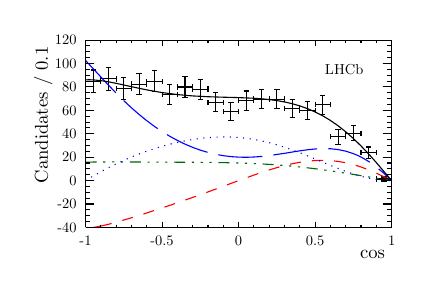
\begin{tikzpicture}
\pgfdeclareplotmark{cross} {
\pgfpathmoveto{\pgfpoint{-0.3\pgfplotmarksize}{\pgfplotmarksize}}
\pgfpathlineto{\pgfpoint{+0.3\pgfplotmarksize}{\pgfplotmarksize}}
\pgfpathlineto{\pgfpoint{+0.3\pgfplotmarksize}{0.3\pgfplotmarksize}}
\pgfpathlineto{\pgfpoint{+1\pgfplotmarksize}{0.3\pgfplotmarksize}}
\pgfpathlineto{\pgfpoint{+1\pgfplotmarksize}{-0.3\pgfplotmarksize}}
\pgfpathlineto{\pgfpoint{+0.3\pgfplotmarksize}{-0.3\pgfplotmarksize}}
\pgfpathlineto{\pgfpoint{+0.3\pgfplotmarksize}{-1.\pgfplotmarksize}}
\pgfpathlineto{\pgfpoint{-0.3\pgfplotmarksize}{-1.\pgfplotmarksize}}
\pgfpathlineto{\pgfpoint{-0.3\pgfplotmarksize}{-0.3\pgfplotmarksize}}
\pgfpathlineto{\pgfpoint{-1.\pgfplotmarksize}{-0.3\pgfplotmarksize}}
\pgfpathlineto{\pgfpoint{-1.\pgfplotmarksize}{0.3\pgfplotmarksize}}
\pgfpathlineto{\pgfpoint{-0.3\pgfplotmarksize}{0.3\pgfplotmarksize}}
\pgfpathclose
\pgfusepathqstroke
}
\pgfdeclareplotmark{cross*} {
\pgfpathmoveto{\pgfpoint{-0.3\pgfplotmarksize}{\pgfplotmarksize}}
\pgfpathlineto{\pgfpoint{+0.3\pgfplotmarksize}{\pgfplotmarksize}}
\pgfpathlineto{\pgfpoint{+0.3\pgfplotmarksize}{0.3\pgfplotmarksize}}
\pgfpathlineto{\pgfpoint{+1\pgfplotmarksize}{0.3\pgfplotmarksize}}
\pgfpathlineto{\pgfpoint{+1\pgfplotmarksize}{-0.3\pgfplotmarksize}}
\pgfpathlineto{\pgfpoint{+0.3\pgfplotmarksize}{-0.3\pgfplotmarksize}}
\pgfpathlineto{\pgfpoint{+0.3\pgfplotmarksize}{-1.\pgfplotmarksize}}
\pgfpathlineto{\pgfpoint{-0.3\pgfplotmarksize}{-1.\pgfplotmarksize}}
\pgfpathlineto{\pgfpoint{-0.3\pgfplotmarksize}{-0.3\pgfplotmarksize}}
\pgfpathlineto{\pgfpoint{-1.\pgfplotmarksize}{-0.3\pgfplotmarksize}}
\pgfpathlineto{\pgfpoint{-1.\pgfplotmarksize}{0.3\pgfplotmarksize}}
\pgfpathlineto{\pgfpoint{-0.3\pgfplotmarksize}{0.3\pgfplotmarksize}}
\pgfpathclose
\pgfusepathqfillstroke
}
\pgfdeclareplotmark{newstar} {
\pgfpathmoveto{\pgfqpoint{0pt}{\pgfplotmarksize}}
\pgfpathlineto{\pgfqpointpolar{44}{0.5\pgfplotmarksize}}
\pgfpathlineto{\pgfqpointpolar{18}{\pgfplotmarksize}}
\pgfpathlineto{\pgfqpointpolar{-20}{0.5\pgfplotmarksize}}
\pgfpathlineto{\pgfqpointpolar{-54}{\pgfplotmarksize}}
\pgfpathlineto{\pgfqpointpolar{-90}{0.5\pgfplotmarksize}}
\pgfpathlineto{\pgfqpointpolar{234}{\pgfplotmarksize}}
\pgfpathlineto{\pgfqpointpolar{198}{0.5\pgfplotmarksize}}
\pgfpathlineto{\pgfqpointpolar{162}{\pgfplotmarksize}}
\pgfpathlineto{\pgfqpointpolar{134}{0.5\pgfplotmarksize}}
\pgfpathclose
\pgfusepathqstroke
}
\pgfdeclareplotmark{newstar*} {
\pgfpathmoveto{\pgfqpoint{0pt}{\pgfplotmarksize}}
\pgfpathlineto{\pgfqpointpolar{44}{0.5\pgfplotmarksize}}
\pgfpathlineto{\pgfqpointpolar{18}{\pgfplotmarksize}}
\pgfpathlineto{\pgfqpointpolar{-20}{0.5\pgfplotmarksize}}
\pgfpathlineto{\pgfqpointpolar{-54}{\pgfplotmarksize}}
\pgfpathlineto{\pgfqpointpolar{-90}{0.5\pgfplotmarksize}}
\pgfpathlineto{\pgfqpointpolar{234}{\pgfplotmarksize}}
\pgfpathlineto{\pgfqpointpolar{198}{0.5\pgfplotmarksize}}
\pgfpathlineto{\pgfqpointpolar{162}{\pgfplotmarksize}}
\pgfpathlineto{\pgfqpointpolar{134}{0.5\pgfplotmarksize}}
\pgfpathclose
\pgfusepathqfillstroke
}
\definecolor{c}{rgb}{1,1,1};
\draw [color=c, fill=c] (0.1,3.20034) rectangle (4.9,6.21242);
\draw [color=c, fill=c] (0.772,3.68227) rectangle (4.66,6.06181);
\definecolor{c}{rgb}{0,0,0};
\draw [c] (0.772,3.68227) -- (0.772,6.06181) -- (4.66,6.06181) -- (4.66,3.68227) -- (0.772,3.68227);
\definecolor{c}{rgb}{1,1,1};
\draw [color=c, fill=c] (0.772,3.68227) rectangle (4.66,6.06181);
\definecolor{c}{rgb}{0,0,0};
\draw [c] (0.772,3.68227) -- (0.772,6.06181) -- (4.66,6.06181) -- (4.66,3.68227) -- (0.772,3.68227);
\draw [c,line width=0.4] (0.772,3.68227) -- (4.66,3.68227);
\draw [anchor= east] (4.66,3.34492) node[scale=0.672711, rotate=0]{$\cos\thetaK$};
\draw [c,line width=0.4] (0.772,3.75546) -- (0.772,3.68227);
\draw [c,line width=0.4] (0.9664,3.71887) -- (0.9664,3.68227);
\draw [c,line width=0.4] (1.1608,3.71887) -- (1.1608,3.68227);
\draw [c,line width=0.4] (1.3552,3.71887) -- (1.3552,3.68227);
\draw [c,line width=0.4] (1.5496,3.71887) -- (1.5496,3.68227);
\draw [c,line width=0.4] (1.744,3.75546) -- (1.744,3.68227);
\draw [c,line width=0.4] (1.9384,3.71887) -- (1.9384,3.68227);
\draw [c,line width=0.4] (2.1328,3.71887) -- (2.1328,3.68227);
\draw [c,line width=0.4] (2.3272,3.71887) -- (2.3272,3.68227);
\draw [c,line width=0.4] (2.5216,3.71887) -- (2.5216,3.68227);
\draw [c,line width=0.4] (2.716,3.75546) -- (2.716,3.68227);
\draw [c,line width=0.4] (2.9104,3.71887) -- (2.9104,3.68227);
\draw [c,line width=0.4] (3.1048,3.71887) -- (3.1048,3.68227);
\draw [c,line width=0.4] (3.2992,3.71887) -- (3.2992,3.68227);
\draw [c,line width=0.4] (3.4936,3.71887) -- (3.4936,3.68227);
\draw [c,line width=0.4] (3.688,3.75546) -- (3.688,3.68227);
\draw [c,line width=0.4] (3.8824,3.71887) -- (3.8824,3.68227);
\draw [c,line width=0.4] (4.0768,3.71887) -- (4.0768,3.68227);
\draw [c,line width=0.4] (4.2712,3.71887) -- (4.2712,3.68227);
\draw [c,line width=0.4] (4.4656,3.71887) -- (4.4656,3.68227);
\draw [c,line width=0.4] (4.66,3.75546) -- (4.66,3.68227);
\draw [anchor=base] (0.772,3.45937) node[scale=0.52322, rotate=0]{-1};
\draw [anchor=base] (1.744,3.45937) node[scale=0.52322, rotate=0]{-0.5};
\draw [anchor=base] (2.716,3.45937) node[scale=0.52322, rotate=0]{0};
\draw [anchor=base] (3.688,3.45937) node[scale=0.52322, rotate=0]{0.5};
\draw [anchor=base] (4.66,3.45937) node[scale=0.52322, rotate=0]{1};
\draw [c,line width=0.4] (0.772,6.06181) -- (4.66,6.06181);
\draw [c,line width=0.4] (0.772,5.98862) -- (0.772,6.06181);
\draw [c,line width=0.4] (0.9664,6.02522) -- (0.9664,6.06181);
\draw [c,line width=0.4] (1.1608,6.02522) -- (1.1608,6.06181);
\draw [c,line width=0.4] (1.3552,6.02522) -- (1.3552,6.06181);
\draw [c,line width=0.4] (1.5496,6.02522) -- (1.5496,6.06181);
\draw [c,line width=0.4] (1.744,5.98862) -- (1.744,6.06181);
\draw [c,line width=0.4] (1.9384,6.02522) -- (1.9384,6.06181);
\draw [c,line width=0.4] (2.1328,6.02522) -- (2.1328,6.06181);
\draw [c,line width=0.4] (2.3272,6.02522) -- (2.3272,6.06181);
\draw [c,line width=0.4] (2.5216,6.02522) -- (2.5216,6.06181);
\draw [c,line width=0.4] (2.716,5.98862) -- (2.716,6.06181);
\draw [c,line width=0.4] (2.9104,6.02522) -- (2.9104,6.06181);
\draw [c,line width=0.4] (3.1048,6.02522) -- (3.1048,6.06181);
\draw [c,line width=0.4] (3.2992,6.02522) -- (3.2992,6.06181);
\draw [c,line width=0.4] (3.4936,6.02522) -- (3.4936,6.06181);
\draw [c,line width=0.4] (3.688,5.98862) -- (3.688,6.06181);
\draw [c,line width=0.4] (3.8824,6.02522) -- (3.8824,6.06181);
\draw [c,line width=0.4] (4.0768,6.02522) -- (4.0768,6.06181);
\draw [c,line width=0.4] (4.2712,6.02522) -- (4.2712,6.06181);
\draw [c,line width=0.4] (4.4656,6.02522) -- (4.4656,6.06181);
\draw [c,line width=0.4] (4.66,5.98862) -- (4.66,6.06181);
\draw [c,line width=0.4] (0.772,3.68227) -- (0.772,6.06181);
\draw [anchor= east] (0.2344,6.06181) node[scale=0.672711, rotate=90]{Candidates / 0.1};
\draw [c,line width=0.4] (0.88576,3.68227) -- (0.772,3.68227);
\draw [c,line width=0.4] (0.82888,3.75663) -- (0.772,3.75663);
\draw [c,line width=0.4] (0.82888,3.83099) -- (0.772,3.83099);
\draw [c,line width=0.4] (0.82888,3.90535) -- (0.772,3.90535);
\draw [c,line width=0.4] (0.88576,3.97971) -- (0.772,3.97971);
\draw [c,line width=0.4] (0.82888,4.05407) -- (0.772,4.05407);
\draw [c,line width=0.4] (0.82888,4.12843) -- (0.772,4.12843);
\draw [c,line width=0.4] (0.82888,4.20279) -- (0.772,4.20279);
\draw [c,line width=0.4] (0.88576,4.27715) -- (0.772,4.27715);
\draw [c,line width=0.4] (0.82888,4.35152) -- (0.772,4.35152);
\draw [c,line width=0.4] (0.82888,4.42588) -- (0.772,4.42588);
\draw [c,line width=0.4] (0.82888,4.50024) -- (0.772,4.50024);
\draw [c,line width=0.4] (0.88576,4.5746) -- (0.772,4.5746);
\draw [c,line width=0.4] (0.82888,4.64896) -- (0.772,4.64896);
\draw [c,line width=0.4] (0.82888,4.72332) -- (0.772,4.72332);
\draw [c,line width=0.4] (0.82888,4.79768) -- (0.772,4.79768);
\draw [c,line width=0.4] (0.88576,4.87204) -- (0.772,4.87204);
\draw [c,line width=0.4] (0.82888,4.9464) -- (0.772,4.9464);
\draw [c,line width=0.4] (0.82888,5.02076) -- (0.772,5.02076);
\draw [c,line width=0.4] (0.82888,5.09512) -- (0.772,5.09512);
\draw [c,line width=0.4] (0.88576,5.16948) -- (0.772,5.16948);
\draw [c,line width=0.4] (0.82888,5.24384) -- (0.772,5.24384);
\draw [c,line width=0.4] (0.82888,5.3182) -- (0.772,5.3182);
\draw [c,line width=0.4] (0.82888,5.39257) -- (0.772,5.39257);
\draw [c,line width=0.4] (0.88576,5.46693) -- (0.772,5.46693);
\draw [c,line width=0.4] (0.82888,5.54129) -- (0.772,5.54129);
\draw [c,line width=0.4] (0.82888,5.61565) -- (0.772,5.61565);
\draw [c,line width=0.4] (0.82888,5.69001) -- (0.772,5.69001);
\draw [c,line width=0.4] (0.88576,5.76437) -- (0.772,5.76437);
\draw [c,line width=0.4] (0.82888,5.83873) -- (0.772,5.83873);
\draw [c,line width=0.4] (0.82888,5.91309) -- (0.772,5.91309);
\draw [c,line width=0.4] (0.82888,5.98745) -- (0.772,5.98745);
\draw [c,line width=0.4] (0.88576,6.06181) -- (0.772,6.06181);
\draw [anchor= east] (0.724,3.68227) node[scale=0.52322, rotate=0]{-40};
\draw [anchor= east] (0.724,3.97971) node[scale=0.52322, rotate=0]{-20};
\draw [anchor= east] (0.724,4.27715) node[scale=0.52322, rotate=0]{0};
\draw [anchor= east] (0.724,4.5746) node[scale=0.52322, rotate=0]{20};
\draw [anchor= east] (0.724,4.87204) node[scale=0.52322, rotate=0]{40};
\draw [anchor= east] (0.724,5.16948) node[scale=0.52322, rotate=0]{60};
\draw [anchor= east] (0.724,5.46693) node[scale=0.52322, rotate=0]{80};
\draw [anchor= east] (0.724,5.76437) node[scale=0.52322, rotate=0]{100};
\draw [anchor= east] (0.724,6.06181) node[scale=0.52322, rotate=0]{120};
\draw [c,line width=0.4] (4.66,3.68227) -- (4.66,6.06181);
\draw [c,line width=0.4] (4.54624,3.68227) -- (4.66,3.68227);
\draw [c,line width=0.4] (4.60312,3.75663) -- (4.66,3.75663);
\draw [c,line width=0.4] (4.60312,3.83099) -- (4.66,3.83099);
\draw [c,line width=0.4] (4.60312,3.90535) -- (4.66,3.90535);
\draw [c,line width=0.4] (4.54624,3.97971) -- (4.66,3.97971);
\draw [c,line width=0.4] (4.60312,4.05407) -- (4.66,4.05407);
\draw [c,line width=0.4] (4.60312,4.12843) -- (4.66,4.12843);
\draw [c,line width=0.4] (4.60312,4.20279) -- (4.66,4.20279);
\draw [c,line width=0.4] (4.54624,4.27715) -- (4.66,4.27715);
\draw [c,line width=0.4] (4.60312,4.35152) -- (4.66,4.35152);
\draw [c,line width=0.4] (4.60312,4.42588) -- (4.66,4.42588);
\draw [c,line width=0.4] (4.60312,4.50024) -- (4.66,4.50024);
\draw [c,line width=0.4] (4.54624,4.5746) -- (4.66,4.5746);
\draw [c,line width=0.4] (4.60312,4.64896) -- (4.66,4.64896);
\draw [c,line width=0.4] (4.60312,4.72332) -- (4.66,4.72332);
\draw [c,line width=0.4] (4.60312,4.79768) -- (4.66,4.79768);
\draw [c,line width=0.4] (4.54624,4.87204) -- (4.66,4.87204);
\draw [c,line width=0.4] (4.60312,4.9464) -- (4.66,4.9464);
\draw [c,line width=0.4] (4.60312,5.02076) -- (4.66,5.02076);
\draw [c,line width=0.4] (4.60312,5.09512) -- (4.66,5.09512);
\draw [c,line width=0.4] (4.54624,5.16948) -- (4.66,5.16948);
\draw [c,line width=0.4] (4.60312,5.24384) -- (4.66,5.24384);
\draw [c,line width=0.4] (4.60312,5.3182) -- (4.66,5.3182);
\draw [c,line width=0.4] (4.60312,5.39257) -- (4.66,5.39257);
\draw [c,line width=0.4] (4.54624,5.46693) -- (4.66,5.46693);
\draw [c,line width=0.4] (4.60312,5.54129) -- (4.66,5.54129);
\draw [c,line width=0.4] (4.60312,5.61565) -- (4.66,5.61565);
\draw [c,line width=0.4] (4.60312,5.69001) -- (4.66,5.69001);
\draw [c,line width=0.4] (4.54624,5.76437) -- (4.66,5.76437);
\draw [c,line width=0.4] (4.60312,5.83873) -- (4.66,5.83873);
\draw [c,line width=0.4] (4.60312,5.91309) -- (4.66,5.91309);
\draw [c,line width=0.4] (4.60312,5.98745) -- (4.66,5.98745);
\draw [c,line width=0.4] (4.54624,6.06181) -- (4.66,6.06181);
\draw [c] (0.8692,5.53998) -- (0.772,5.53998);
\draw [c] (0.772,5.50643) -- (0.772,5.57354);
\draw [c] (0.8692,5.53998) -- (0.9664,5.53998);
\draw [c] (0.9664,5.50643) -- (0.9664,5.57354);
\draw [c] (0.8692,5.53998) -- (0.8692,5.68166);
\draw [c] (0.835643,5.68166) -- (0.902757,5.68166);
\draw [c] (0.8692,5.53998) -- (0.8692,5.39831);
\draw [c] (0.835643,5.39831) -- (0.902757,5.39831);
\draw [c] (1.0636,5.56842) -- (0.9664,5.56842);
\draw [c] (0.9664,5.53486) -- (0.9664,5.60197);
\draw [c] (1.0636,5.56842) -- (1.1608,5.56842);
\draw [c] (1.1608,5.53486) -- (1.1608,5.60197);
\draw [c] (1.0636,5.56842) -- (1.0636,5.70972);
\draw [c] (1.03004,5.70972) -- (1.09716,5.70972);
\draw [c] (1.0636,5.56842) -- (1.0636,5.42711);
\draw [c] (1.03004,5.42711) -- (1.09716,5.42711);
\draw [c] (1.258,5.44696) -- (1.1608,5.44696);
\draw [c] (1.1608,5.4134) -- (1.1608,5.48052);
\draw [c] (1.258,5.44696) -- (1.3552,5.44696);
\draw [c] (1.3552,5.4134) -- (1.3552,5.48052);
\draw [c] (1.258,5.44696) -- (1.258,5.58349);
\draw [c] (1.22444,5.58349) -- (1.29156,5.58349);
\draw [c] (1.258,5.44696) -- (1.258,5.31043);
\draw [c] (1.22444,5.31043) -- (1.29156,5.31043);
\draw [c] (1.4524,5.50273) -- (1.3552,5.50273);
\draw [c] (1.3552,5.46918) -- (1.3552,5.53629);
\draw [c] (1.4524,5.50273) -- (1.5496,5.50273);
\draw [c] (1.5496,5.46918) -- (1.5496,5.53629);
\draw [c] (1.4524,5.50273) -- (1.4524,5.63754);
\draw [c] (1.41884,5.63754) -- (1.48596,5.63754);
\draw [c] (1.4524,5.50273) -- (1.4524,5.36793);
\draw [c] (1.41884,5.36793) -- (1.48596,5.36793);
\draw [c] (1.6468,5.53811) -- (1.5496,5.53811);
\draw [c] (1.5496,5.50455) -- (1.5496,5.57166);
\draw [c] (1.6468,5.53811) -- (1.744,5.53811);
\draw [c] (1.744,5.50455) -- (1.744,5.57166);
\draw [c] (1.6468,5.53811) -- (1.6468,5.67306);
\draw [c] (1.61324,5.67306) -- (1.68036,5.67306);
\draw [c] (1.6468,5.53811) -- (1.6468,5.40315);
\draw [c] (1.61324,5.40315) -- (1.68036,5.40315);
\draw [c] (1.8412,5.3681) -- (1.744,5.3681);
\draw [c] (1.744,5.33454) -- (1.744,5.40165);
\draw [c] (1.8412,5.3681) -- (1.9384,5.3681);
\draw [c] (1.9384,5.33454) -- (1.9384,5.40165);
\draw [c] (1.8412,5.3681) -- (1.8412,5.49512);
\draw [c] (1.80764,5.49512) -- (1.87476,5.49512);
\draw [c] (1.8412,5.3681) -- (1.8412,5.24107);
\draw [c] (1.80764,5.24107) -- (1.87476,5.24107);
\draw [c] (2.0356,5.4665) -- (1.9384,5.4665);
\draw [c] (1.9384,5.43295) -- (1.9384,5.50006);
\draw [c] (2.0356,5.4665) -- (2.1328,5.4665);
\draw [c] (2.1328,5.43295) -- (2.1328,5.50006);
\draw [c] (2.0356,5.4665) -- (2.0356,5.59827);
\draw [c] (2.00204,5.59827) -- (2.06916,5.59827);
\draw [c] (2.0356,5.4665) -- (2.0356,5.33473);
\draw [c] (2.00204,5.33473) -- (2.06916,5.33473);
\draw [c] (2.23,5.43953) -- (2.1328,5.43953);
\draw [c] (2.1328,5.40597) -- (2.1328,5.47309);
\draw [c] (2.23,5.43953) -- (2.3272,5.43953);
\draw [c] (2.3272,5.40597) -- (2.3272,5.47309);
\draw [c] (2.23,5.43953) -- (2.23,5.56678);
\draw [c] (2.19644,5.56678) -- (2.26356,5.56678);
\draw [c] (2.23,5.43953) -- (2.23,5.31228);
\draw [c] (2.19644,5.31228) -- (2.26356,5.31228);
\draw [c] (2.4244,5.2713) -- (2.3272,5.2713);
\draw [c] (2.3272,5.23774) -- (2.3272,5.30485);
\draw [c] (2.4244,5.2713) -- (2.5216,5.2713);
\draw [c] (2.5216,5.23774) -- (2.5216,5.30485);
\draw [c] (2.4244,5.2713) -- (2.4244,5.39227);
\draw [c] (2.39084,5.39227) -- (2.45796,5.39227);
\draw [c] (2.4244,5.2713) -- (2.4244,5.15033);
\draw [c] (2.39084,5.15033) -- (2.45796,5.15033);
\draw [c] (2.6188,5.15486) -- (2.5216,5.15486);
\draw [c] (2.5216,5.1213) -- (2.5216,5.18842);
\draw [c] (2.6188,5.15486) -- (2.716,5.15486);
\draw [c] (2.716,5.1213) -- (2.716,5.18842);
\draw [c] (2.6188,5.15486) -- (2.6188,5.26834);
\draw [c] (2.58524,5.26834) -- (2.65236,5.26834);
\draw [c] (2.6188,5.15486) -- (2.6188,5.04137);
\draw [c] (2.58524,5.04137) -- (2.65236,5.04137);
\draw [c] (2.8132,5.29357) -- (2.716,5.29357);
\draw [c] (2.716,5.26001) -- (2.716,5.32713);
\draw [c] (2.8132,5.29357) -- (2.9104,5.29357);
\draw [c] (2.9104,5.26001) -- (2.9104,5.32713);
\draw [c] (2.8132,5.29357) -- (2.8132,5.41525);
\draw [c] (2.77964,5.41525) -- (2.84676,5.41525);
\draw [c] (2.8132,5.29357) -- (2.8132,5.17189);
\draw [c] (2.77964,5.17189) -- (2.84676,5.17189);
\draw [c] (3.0076,5.31225) -- (2.9104,5.31225);
\draw [c] (2.9104,5.2787) -- (2.9104,5.34581);
\draw [c] (3.0076,5.31225) -- (3.1048,5.31225);
\draw [c] (3.1048,5.2787) -- (3.1048,5.34581);
\draw [c] (3.0076,5.31225) -- (3.0076,5.43309);
\draw [c] (2.97404,5.43309) -- (3.04116,5.43309);
\draw [c] (3.0076,5.31225) -- (3.0076,5.19142);
\draw [c] (2.97404,5.19142) -- (3.04116,5.19142);
\draw [c] (3.202,5.31224) -- (3.1048,5.31224);
\draw [c] (3.1048,5.27868) -- (3.1048,5.3458);
\draw [c] (3.202,5.31224) -- (3.2992,5.31224);
\draw [c] (3.2992,5.27868) -- (3.2992,5.3458);
\draw [c] (3.202,5.31224) -- (3.202,5.43256);
\draw [c] (3.16844,5.43256) -- (3.23556,5.43256);
\draw [c] (3.202,5.31224) -- (3.202,5.19192);
\draw [c] (3.16844,5.19192) -- (3.23556,5.19192);
\draw [c] (3.3964,5.19601) -- (3.2992,5.19601);
\draw [c] (3.2992,5.16245) -- (3.2992,5.22957);
\draw [c] (3.3964,5.19601) -- (3.4936,5.19601);
\draw [c] (3.4936,5.16245) -- (3.4936,5.22957);
\draw [c] (3.3964,5.19601) -- (3.3964,5.31245);
\draw [c] (3.36284,5.31245) -- (3.42996,5.31245);
\draw [c] (3.3964,5.19601) -- (3.3964,5.07958);
\draw [c] (3.36284,5.07958) -- (3.42996,5.07958);
\draw [c] (3.5908,5.16841) -- (3.4936,5.16841);
\draw [c] (3.4936,5.13485) -- (3.4936,5.20197);
\draw [c] (3.5908,5.16841) -- (3.688,5.16841);
\draw [c] (3.688,5.13485) -- (3.688,5.20197);
\draw [c] (3.5908,5.16841) -- (3.5908,5.28525);
\draw [c] (3.55724,5.28525) -- (3.62436,5.28525);
\draw [c] (3.5908,5.16841) -- (3.5908,5.05158);
\draw [c] (3.55724,5.05158) -- (3.62436,5.05158);
\draw [c] (3.7852,5.24155) -- (3.688,5.24155);
\draw [c] (3.688,5.208) -- (3.688,5.27511);
\draw [c] (3.7852,5.24155) -- (3.8824,5.24155);
\draw [c] (3.8824,5.208) -- (3.8824,5.27511);
\draw [c] (3.7852,5.24155) -- (3.7852,5.36086);
\draw [c] (3.75164,5.36086) -- (3.81876,5.36086);
\draw [c] (3.7852,5.24155) -- (3.7852,5.12225);
\draw [c] (3.75164,5.12225) -- (3.81876,5.12225);
\draw [c] (3.9796,4.83424) -- (3.8824,4.83424);
\draw [c] (3.8824,4.80068) -- (3.8824,4.86779);
\draw [c] (3.9796,4.83424) -- (4.0768,4.83424);
\draw [c] (4.0768,4.80068) -- (4.0768,4.86779);
\draw [c] (3.9796,4.83424) -- (3.9796,4.92924);
\draw [c] (3.94604,4.92924) -- (4.01316,4.92924);
\draw [c] (3.9796,4.83424) -- (3.9796,4.73924);
\draw [c] (3.94604,4.73924) -- (4.01316,4.73924);
\draw [c] (4.174,4.87912) -- (4.0768,4.87912);
\draw [c] (4.0768,4.84557) -- (4.0768,4.91268);
\draw [c] (4.174,4.87912) -- (4.2712,4.87912);
\draw [c] (4.2712,4.84557) -- (4.2712,4.91268);
\draw [c] (4.174,4.87912) -- (4.174,4.97502);
\draw [c] (4.14044,4.97502) -- (4.20756,4.97502);
\draw [c] (4.174,4.87912) -- (4.174,4.78323);
\draw [c] (4.14044,4.78323) -- (4.20756,4.78323);
\draw [c] (4.3684,4.63391) -- (4.2712,4.63391);
\draw [c] (4.2712,4.60035) -- (4.2712,4.66747);
\draw [c] (4.3684,4.63391) -- (4.4656,4.63391);
\draw [c] (4.4656,4.60035) -- (4.4656,4.66747);
\draw [c] (4.3684,4.63391) -- (4.3684,4.70429);
\draw [c] (4.33484,4.70429) -- (4.40196,4.70429);
\draw [c] (4.3684,4.63391) -- (4.3684,4.56353);
\draw [c] (4.33484,4.56353) -- (4.40196,4.56353);
\draw [c] (4.5628,4.29753) -- (4.4656,4.29753);
\draw [c] (4.4656,4.26397) -- (4.4656,4.33109);
\draw [c] (4.5628,4.29753) -- (4.66,4.29753);
\draw [c] (4.66,4.26397) -- (4.66,4.33109);
\draw [c] (4.5628,4.29753) -- (4.5628,4.32295);
\draw [c] (4.52924,4.32295) -- (4.59636,4.32295);
\draw [c] (4.5628,4.29753) -- (4.5628,4.27211);
\draw [c] (4.52924,4.27211) -- (4.59636,4.27211);
\foreach \P in
 {(0.8692,5.53998),(1.0636,5.56842),(1.258,5.44696),(1.4524,5.50273),(1.6468,5.53811),(1.8412,5.3681),(2.0356,5.4665),(2.23,5.43953),(2.4244,5.2713),(2.6188,5.15486),(2.8132,5.29357),(3.0076,5.31225),(3.202,5.31224),(3.3964,5.19601),(3.5908,5.16841),
(3.7852,5.24155),(3.9796,4.83424),(4.174,4.87912),(4.3684,4.63391),(4.5628,4.29753)}{\draw[mark options={color=c,fill=c},mark size=1.201201pt,mark=] plot coordinates {\P};}
\definecolor{c}{rgb}{1,0,0};
\draw [c,dash pattern=on 4pt off 4pt] (0.873342,3.68227) -- (0.9664,3.69993);
\draw [c,dash pattern=on 4pt off 4pt] (0.9664,3.69993) -- (1.0636,3.7225) -- (1.1608,3.74806) -- (1.3552,3.80497) -- (1.5496,3.86625) -- (1.744,3.92998) -- (1.9384,3.99564) -- (2.1328,4.06338) -- (2.3272,4.1333) -- (2.5216,4.20499) -- (2.716,4.27715)
 -- (2.9104,4.34749) -- (3.0076,4.38096) -- (3.1048,4.41264) -- (3.202,4.44198) -- (3.2992,4.46838) -- (3.3964,4.49122) -- (3.4936,4.50989) -- (3.5908,4.52378) -- (3.688,4.53231) -- (3.7852,4.53498) -- (3.8824,4.53134) -- (3.9796,4.52108) --
 (4.0768,4.50403) -- (4.174,4.4802) -- (4.2712,4.44982) -- (4.3684,4.41337) -- (4.4656,4.37163) -- (4.5628,4.32572) -- (4.66,4.27715) -- (4.66,4.27715) -- (4.66,4.27715);
\definecolor{c}{rgb}{0,0.4,0};
\draw [c,dash pattern=on 4pt off 2.4pt on 0.8pt off 2.4pt on 0.8pt off 2.4pt on 0.8pt off 2.4pt] (0.772,4.511) -- (0.772,4.511);
\draw [c,dash pattern=on 4pt off 2.4pt on 0.8pt off 2.4pt on 0.8pt off 2.4pt on 0.8pt off 2.4pt] (0.772,4.511) -- (0.8692,4.51284) -- (0.9664,4.51387) -- (1.1608,4.51432) -- (1.3552,4.51364) -- (1.5496,4.51264) -- (1.744,4.5117) -- (1.9384,4.51088)
 -- (2.1328,4.50991) -- (2.3272,4.50835) -- (2.5216,4.50557) -- (2.6188,4.50351) -- (2.716,4.50089) -- (2.8132,4.49762) -- (2.9104,4.49361) -- (3.0076,4.48879) -- (3.1048,4.48308) -- (3.202,4.47643) -- (3.2992,4.46878) -- (3.3964,4.46011) --
 (3.4936,4.45039) -- (3.5908,4.43962) -- (3.688,4.42783) -- (3.7852,4.41506) -- (3.8824,4.40138) -- (3.9796,4.38688) -- (4.0768,4.37168) -- (4.2712,4.33987) -- (4.4656,4.30761) -- (4.5628,4.29199) -- (4.66,4.27715) -- (4.66,4.27715) --
 (4.66,4.27715);
\definecolor{c}{rgb}{0,0,1};
\draw [c,dotted] (0.772,4.27715) -- (0.772,4.27715);
\draw [c,dotted] (0.772,4.27715) -- (0.8692,4.33452) -- (0.9664,4.38926) -- (1.0636,4.44099) -- (1.1608,4.4895) -- (1.258,4.53471) -- (1.3552,4.57663) -- (1.4524,4.6153) -- (1.5496,4.65081) -- (1.6468,4.68322) -- (1.744,4.71258) -- (1.8412,4.73891)
 -- (1.9384,4.76217) -- (2.0356,4.78232) -- (2.1328,4.79925) -- (2.23,4.81282) -- (2.3272,4.82288) -- (2.4244,4.82925) -- (2.5216,4.83174) -- (2.6188,4.8302) -- (2.716,4.82448) -- (2.8132,4.81447) -- (2.9104,4.80014) -- (3.0076,4.78149) --
 (3.1048,4.75863) -- (3.202,4.73176) -- (3.2992,4.70118) -- (3.3964,4.66728) -- (3.4936,4.63061) -- (3.5908,4.59178) -- (3.688,4.55154) -- (3.8824,4.47027) -- (3.9796,4.43117) -- (4.0768,4.39444) -- (4.174,4.36113) -- (4.2226,4.34607) --
 (4.2712,4.33225) -- (4.3198,4.31976) -- (4.3684,4.30872) -- (4.417,4.29922) -- (4.4656,4.29134) -- (4.5142,4.28516) -- (4.5628,4.28071) -- (4.6114,4.27804) -- (4.66,4.27715) -- (4.66,4.27715) -- (4.66,4.27715);
\draw [c,dash pattern=on 16pt off 4pt] (0.772,5.80367) -- (0.772,5.80367);
\draw [c,dash pattern=on 16pt off 4pt] (0.772,5.80367) -- (0.9664,5.59361) -- (1.0636,5.48951) -- (1.1608,5.38871) -- (1.258,5.29251) -- (1.3552,5.20174) -- (1.4524,5.11692) -- (1.5496,5.03835) -- (1.6468,4.96614) -- (1.744,4.9003) --
 (1.8412,4.84078) -- (1.9384,4.78749) -- (2.0356,4.74036) -- (2.1328,4.69928) -- (2.23,4.66418) -- (2.3272,4.63499) -- (2.4244,4.61162) -- (2.5216,4.59396) -- (2.6188,4.58188) -- (2.716,4.57517) -- (2.8132,4.57355) -- (2.9104,4.57664) --
 (3.0076,4.58393) -- (3.1048,4.59478) -- (3.2992,4.6238) -- (3.4936,4.65542) -- (3.5908,4.66894) -- (3.688,4.67892) -- (3.7852,4.68376) -- (3.8824,4.6818) -- (3.9796,4.67143) -- (4.0768,4.65115) -- (4.174,4.61963) -- (4.2226,4.59933) --
 (4.2712,4.57587) -- (4.3198,4.54921) -- (4.3684,4.51932) -- (4.417,4.48623) -- (4.4656,4.45001) -- (4.5628,4.3687) -- (4.66,4.27715) -- (4.66,4.27715) -- (4.66,4.27715);
\definecolor{c}{rgb}{0,0,0};
\draw [c] (0.772,5.55672) -- (0.772,5.55672);
\draw [c] (0.772,5.55672) -- (0.8206,5.55778) -- (0.8692,5.55621) -- (0.9664,5.54686) -- (1.0636,5.53152) -- (1.1608,5.51249) -- (1.3552,5.47008) -- (1.5496,5.42932) -- (1.744,5.39523) -- (1.9384,5.36972) -- (2.1328,5.35261) -- (2.3272,5.34235) --
 (2.5216,5.33639) -- (2.716,5.33133) -- (2.9104,5.32302) -- (3.0076,5.31614) -- (3.1048,5.30653) -- (3.202,5.29347) -- (3.2992,5.27621) -- (3.3964,5.25395) -- (3.4936,5.22591) -- (3.5908,5.19131) -- (3.688,5.14939) -- (3.7852,5.0995) --
 (3.8824,5.04106) -- (3.9796,4.97365) -- (4.0768,4.89707) -- (4.174,4.81137) -- (4.2712,4.71696) -- (4.3684,4.61466) -- (4.4656,4.50583) -- (4.66,4.27715) -- (4.66,4.27715) -- (4.66,4.27715);
\draw [c,line width=0.4] (0.772,3.68227) -- (4.66,3.68227);
\draw [c,line width=0.4] (0.772,3.75546) -- (0.772,3.68227);
\draw [c,line width=0.4] (0.9664,3.71887) -- (0.9664,3.68227);
\draw [c,line width=0.4] (1.1608,3.71887) -- (1.1608,3.68227);
\draw [c,line width=0.4] (1.3552,3.71887) -- (1.3552,3.68227);
\draw [c,line width=0.4] (1.5496,3.71887) -- (1.5496,3.68227);
\draw [c,line width=0.4] (1.744,3.75546) -- (1.744,3.68227);
\draw [c,line width=0.4] (1.9384,3.71887) -- (1.9384,3.68227);
\draw [c,line width=0.4] (2.1328,3.71887) -- (2.1328,3.68227);
\draw [c,line width=0.4] (2.3272,3.71887) -- (2.3272,3.68227);
\draw [c,line width=0.4] (2.5216,3.71887) -- (2.5216,3.68227);
\draw [c,line width=0.4] (2.716,3.75546) -- (2.716,3.68227);
\draw [c,line width=0.4] (2.9104,3.71887) -- (2.9104,3.68227);
\draw [c,line width=0.4] (3.1048,3.71887) -- (3.1048,3.68227);
\draw [c,line width=0.4] (3.2992,3.71887) -- (3.2992,3.68227);
\draw [c,line width=0.4] (3.4936,3.71887) -- (3.4936,3.68227);
\draw [c,line width=0.4] (3.688,3.75546) -- (3.688,3.68227);
\draw [c,line width=0.4] (3.8824,3.71887) -- (3.8824,3.68227);
\draw [c,line width=0.4] (4.0768,3.71887) -- (4.0768,3.68227);
\draw [c,line width=0.4] (4.2712,3.71887) -- (4.2712,3.68227);
\draw [c,line width=0.4] (4.4656,3.71887) -- (4.4656,3.68227);
\draw [c,line width=0.4] (4.66,3.75546) -- (4.66,3.68227);
\draw [c,line width=0.4] (0.772,6.06181) -- (4.66,6.06181);
\draw [c,line width=0.4] (0.772,5.98862) -- (0.772,6.06181);
\draw [c,line width=0.4] (0.9664,6.02522) -- (0.9664,6.06181);
\draw [c,line width=0.4] (1.1608,6.02522) -- (1.1608,6.06181);
\draw [c,line width=0.4] (1.3552,6.02522) -- (1.3552,6.06181);
\draw [c,line width=0.4] (1.5496,6.02522) -- (1.5496,6.06181);
\draw [c,line width=0.4] (1.744,5.98862) -- (1.744,6.06181);
\draw [c,line width=0.4] (1.9384,6.02522) -- (1.9384,6.06181);
\draw [c,line width=0.4] (2.1328,6.02522) -- (2.1328,6.06181);
\draw [c,line width=0.4] (2.3272,6.02522) -- (2.3272,6.06181);
\draw [c,line width=0.4] (2.5216,6.02522) -- (2.5216,6.06181);
\draw [c,line width=0.4] (2.716,5.98862) -- (2.716,6.06181);
\draw [c,line width=0.4] (2.9104,6.02522) -- (2.9104,6.06181);
\draw [c,line width=0.4] (3.1048,6.02522) -- (3.1048,6.06181);
\draw [c,line width=0.4] (3.2992,6.02522) -- (3.2992,6.06181);
\draw [c,line width=0.4] (3.4936,6.02522) -- (3.4936,6.06181);
\draw [c,line width=0.4] (3.688,5.98862) -- (3.688,6.06181);
\draw [c,line width=0.4] (3.8824,6.02522) -- (3.8824,6.06181);
\draw [c,line width=0.4] (4.0768,6.02522) -- (4.0768,6.06181);
\draw [c,line width=0.4] (4.2712,6.02522) -- (4.2712,6.06181);
\draw [c,line width=0.4] (4.4656,6.02522) -- (4.4656,6.06181);
\draw [c,line width=0.4] (4.66,5.98862) -- (4.66,6.06181);
\draw [c,line width=0.4] (0.772,3.68227) -- (0.772,6.06181);
\draw [c,line width=0.4] (0.88576,3.68227) -- (0.772,3.68227);
\draw [c,line width=0.4] (0.82888,3.75663) -- (0.772,3.75663);
\draw [c,line width=0.4] (0.82888,3.83099) -- (0.772,3.83099);
\draw [c,line width=0.4] (0.82888,3.90535) -- (0.772,3.90535);
\draw [c,line width=0.4] (0.88576,3.97971) -- (0.772,3.97971);
\draw [c,line width=0.4] (0.82888,4.05407) -- (0.772,4.05407);
\draw [c,line width=0.4] (0.82888,4.12843) -- (0.772,4.12843);
\draw [c,line width=0.4] (0.82888,4.20279) -- (0.772,4.20279);
\draw [c,line width=0.4] (0.88576,4.27715) -- (0.772,4.27715);
\draw [c,line width=0.4] (0.82888,4.35152) -- (0.772,4.35152);
\draw [c,line width=0.4] (0.82888,4.42588) -- (0.772,4.42588);
\draw [c,line width=0.4] (0.82888,4.50024) -- (0.772,4.50024);
\draw [c,line width=0.4] (0.88576,4.5746) -- (0.772,4.5746);
\draw [c,line width=0.4] (0.82888,4.64896) -- (0.772,4.64896);
\draw [c,line width=0.4] (0.82888,4.72332) -- (0.772,4.72332);
\draw [c,line width=0.4] (0.82888,4.79768) -- (0.772,4.79768);
\draw [c,line width=0.4] (0.88576,4.87204) -- (0.772,4.87204);
\draw [c,line width=0.4] (0.82888,4.9464) -- (0.772,4.9464);
\draw [c,line width=0.4] (0.82888,5.02076) -- (0.772,5.02076);
\draw [c,line width=0.4] (0.82888,5.09512) -- (0.772,5.09512);
\draw [c,line width=0.4] (0.88576,5.16948) -- (0.772,5.16948);
\draw [c,line width=0.4] (0.82888,5.24384) -- (0.772,5.24384);
\draw [c,line width=0.4] (0.82888,5.3182) -- (0.772,5.3182);
\draw [c,line width=0.4] (0.82888,5.39257) -- (0.772,5.39257);
\draw [c,line width=0.4] (0.88576,5.46693) -- (0.772,5.46693);
\draw [c,line width=0.4] (0.82888,5.54129) -- (0.772,5.54129);
\draw [c,line width=0.4] (0.82888,5.61565) -- (0.772,5.61565);
\draw [c,line width=0.4] (0.82888,5.69001) -- (0.772,5.69001);
\draw [c,line width=0.4] (0.88576,5.76437) -- (0.772,5.76437);
\draw [c,line width=0.4] (0.82888,5.83873) -- (0.772,5.83873);
\draw [c,line width=0.4] (0.82888,5.91309) -- (0.772,5.91309);
\draw [c,line width=0.4] (0.82888,5.98745) -- (0.772,5.98745);
\draw [c,line width=0.4] (0.88576,6.06181) -- (0.772,6.06181);
\draw [c,line width=0.4] (4.66,3.68227) -- (4.66,6.06181);
\draw [c,line width=0.4] (4.54624,3.68227) -- (4.66,3.68227);
\draw [c,line width=0.4] (4.60312,3.75663) -- (4.66,3.75663);
\draw [c,line width=0.4] (4.60312,3.83099) -- (4.66,3.83099);
\draw [c,line width=0.4] (4.60312,3.90535) -- (4.66,3.90535);
\draw [c,line width=0.4] (4.54624,3.97971) -- (4.66,3.97971);
\draw [c,line width=0.4] (4.60312,4.05407) -- (4.66,4.05407);
\draw [c,line width=0.4] (4.60312,4.12843) -- (4.66,4.12843);
\draw [c,line width=0.4] (4.60312,4.20279) -- (4.66,4.20279);
\draw [c,line width=0.4] (4.54624,4.27715) -- (4.66,4.27715);
\draw [c,line width=0.4] (4.60312,4.35152) -- (4.66,4.35152);
\draw [c,line width=0.4] (4.60312,4.42588) -- (4.66,4.42588);
\draw [c,line width=0.4] (4.60312,4.50024) -- (4.66,4.50024);
\draw [c,line width=0.4] (4.54624,4.5746) -- (4.66,4.5746);
\draw [c,line width=0.4] (4.60312,4.64896) -- (4.66,4.64896);
\draw [c,line width=0.4] (4.60312,4.72332) -- (4.66,4.72332);
\draw [c,line width=0.4] (4.60312,4.79768) -- (4.66,4.79768);
\draw [c,line width=0.4] (4.54624,4.87204) -- (4.66,4.87204);
\draw [c,line width=0.4] (4.60312,4.9464) -- (4.66,4.9464);
\draw [c,line width=0.4] (4.60312,5.02076) -- (4.66,5.02076);
\draw [c,line width=0.4] (4.60312,5.09512) -- (4.66,5.09512);
\draw [c,line width=0.4] (4.54624,5.16948) -- (4.66,5.16948);
\draw [c,line width=0.4] (4.60312,5.24384) -- (4.66,5.24384);
\draw [c,line width=0.4] (4.60312,5.3182) -- (4.66,5.3182);
\draw [c,line width=0.4] (4.60312,5.39257) -- (4.66,5.39257);
\draw [c,line width=0.4] (4.54624,5.46693) -- (4.66,5.46693);
\draw [c,line width=0.4] (4.60312,5.54129) -- (4.66,5.54129);
\draw [c,line width=0.4] (4.60312,5.61565) -- (4.66,5.61565);
\draw [c,line width=0.4] (4.60312,5.69001) -- (4.66,5.69001);
\draw [c,line width=0.4] (4.54624,5.76437) -- (4.66,5.76437);
\draw [c,line width=0.4] (4.60312,5.83873) -- (4.66,5.83873);
\draw [c,line width=0.4] (4.60312,5.91309) -- (4.66,5.91309);
\draw [c,line width=0.4] (4.60312,5.98745) -- (4.66,5.98745);
\draw [c,line width=0.4] (4.54624,6.06181) -- (4.66,6.06181);
\draw [anchor= west] (3.748,5.6853) node[scale=0.52322, rotate=0]{LHCb};
\end{tikzpicture}
}
  \end{subfigure}%
  \hfill
  \begin{subfigure}{0.5\textwidth}
    \centering
    \tikzsetnextfilename{angPlot_helcosthetaL}
    \scalebox{1.2}{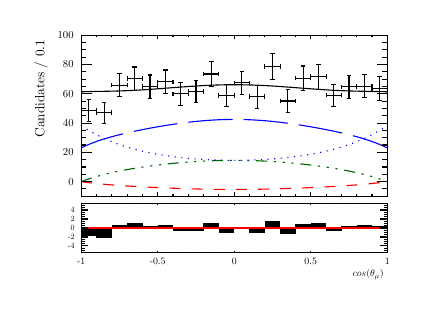
\begin{tikzpicture}
\pgfdeclareplotmark{cross} {
\pgfpathmoveto{\pgfpoint{-0.3\pgfplotmarksize}{\pgfplotmarksize}}
\pgfpathlineto{\pgfpoint{+0.3\pgfplotmarksize}{\pgfplotmarksize}}
\pgfpathlineto{\pgfpoint{+0.3\pgfplotmarksize}{0.3\pgfplotmarksize}}
\pgfpathlineto{\pgfpoint{+1\pgfplotmarksize}{0.3\pgfplotmarksize}}
\pgfpathlineto{\pgfpoint{+1\pgfplotmarksize}{-0.3\pgfplotmarksize}}
\pgfpathlineto{\pgfpoint{+0.3\pgfplotmarksize}{-0.3\pgfplotmarksize}}
\pgfpathlineto{\pgfpoint{+0.3\pgfplotmarksize}{-1.\pgfplotmarksize}}
\pgfpathlineto{\pgfpoint{-0.3\pgfplotmarksize}{-1.\pgfplotmarksize}}
\pgfpathlineto{\pgfpoint{-0.3\pgfplotmarksize}{-0.3\pgfplotmarksize}}
\pgfpathlineto{\pgfpoint{-1.\pgfplotmarksize}{-0.3\pgfplotmarksize}}
\pgfpathlineto{\pgfpoint{-1.\pgfplotmarksize}{0.3\pgfplotmarksize}}
\pgfpathlineto{\pgfpoint{-0.3\pgfplotmarksize}{0.3\pgfplotmarksize}}
\pgfpathclose
\pgfusepathqstroke
}
\pgfdeclareplotmark{cross*} {
\pgfpathmoveto{\pgfpoint{-0.3\pgfplotmarksize}{\pgfplotmarksize}}
\pgfpathlineto{\pgfpoint{+0.3\pgfplotmarksize}{\pgfplotmarksize}}
\pgfpathlineto{\pgfpoint{+0.3\pgfplotmarksize}{0.3\pgfplotmarksize}}
\pgfpathlineto{\pgfpoint{+1\pgfplotmarksize}{0.3\pgfplotmarksize}}
\pgfpathlineto{\pgfpoint{+1\pgfplotmarksize}{-0.3\pgfplotmarksize}}
\pgfpathlineto{\pgfpoint{+0.3\pgfplotmarksize}{-0.3\pgfplotmarksize}}
\pgfpathlineto{\pgfpoint{+0.3\pgfplotmarksize}{-1.\pgfplotmarksize}}
\pgfpathlineto{\pgfpoint{-0.3\pgfplotmarksize}{-1.\pgfplotmarksize}}
\pgfpathlineto{\pgfpoint{-0.3\pgfplotmarksize}{-0.3\pgfplotmarksize}}
\pgfpathlineto{\pgfpoint{-1.\pgfplotmarksize}{-0.3\pgfplotmarksize}}
\pgfpathlineto{\pgfpoint{-1.\pgfplotmarksize}{0.3\pgfplotmarksize}}
\pgfpathlineto{\pgfpoint{-0.3\pgfplotmarksize}{0.3\pgfplotmarksize}}
\pgfpathclose
\pgfusepathqfillstroke
}
\pgfdeclareplotmark{newstar} {
\pgfpathmoveto{\pgfqpoint{0pt}{\pgfplotmarksize}}
\pgfpathlineto{\pgfqpointpolar{44}{0.5\pgfplotmarksize}}
\pgfpathlineto{\pgfqpointpolar{18}{\pgfplotmarksize}}
\pgfpathlineto{\pgfqpointpolar{-20}{0.5\pgfplotmarksize}}
\pgfpathlineto{\pgfqpointpolar{-54}{\pgfplotmarksize}}
\pgfpathlineto{\pgfqpointpolar{-90}{0.5\pgfplotmarksize}}
\pgfpathlineto{\pgfqpointpolar{234}{\pgfplotmarksize}}
\pgfpathlineto{\pgfqpointpolar{198}{0.5\pgfplotmarksize}}
\pgfpathlineto{\pgfqpointpolar{162}{\pgfplotmarksize}}
\pgfpathlineto{\pgfqpointpolar{134}{0.5\pgfplotmarksize}}
\pgfpathclose
\pgfusepathqstroke
}
\pgfdeclareplotmark{newstar*} {
\pgfpathmoveto{\pgfqpoint{0pt}{\pgfplotmarksize}}
\pgfpathlineto{\pgfqpointpolar{44}{0.5\pgfplotmarksize}}
\pgfpathlineto{\pgfqpointpolar{18}{\pgfplotmarksize}}
\pgfpathlineto{\pgfqpointpolar{-20}{0.5\pgfplotmarksize}}
\pgfpathlineto{\pgfqpointpolar{-54}{\pgfplotmarksize}}
\pgfpathlineto{\pgfqpointpolar{-90}{0.5\pgfplotmarksize}}
\pgfpathlineto{\pgfqpointpolar{234}{\pgfplotmarksize}}
\pgfpathlineto{\pgfqpointpolar{198}{0.5\pgfplotmarksize}}
\pgfpathlineto{\pgfqpointpolar{162}{\pgfplotmarksize}}
\pgfpathlineto{\pgfqpointpolar{134}{0.5\pgfplotmarksize}}
\pgfpathclose
\pgfusepathqfillstroke
}
\definecolor{c}{rgb}{1,1,1};
\draw [color=c, fill=c] (5.1,3.47328) rectangle (9.9,6.74224);
\draw [color=c, fill=c] (5.1,4.51934) rectangle (9.9,6.74224);
\draw [color=c, fill=c] (5.772,4.60826) rectangle (9.66,6.65333);
\definecolor{c}{rgb}{0,0,0};
\draw [c] (5.772,4.60826) -- (5.772,6.65333) -- (9.66,6.65333) -- (9.66,4.60826) -- (5.772,4.60826);
\definecolor{c}{rgb}{1,1,1};
\draw [color=c, fill=c] (5.772,4.60826) rectangle (9.66,6.65333);
\definecolor{c}{rgb}{0,0,0};
\draw [c] (5.772,4.60826) -- (5.772,6.65333) -- (9.66,6.65333) -- (9.66,4.60826) -- (5.772,4.60826);
\draw [c,line width=0.4] (5.772,4.60826) -- (9.66,4.60826);
\draw [anchor= east] (9.66,4.36499) node[scale=0.352642, rotate=0]{$cos(\theta_{\mu})$};
\draw [c,line width=0.4] (5.772,4.66228) -- (5.772,4.60826);
\draw [c,line width=0.4] (5.9664,4.63527) -- (5.9664,4.60826);
\draw [c,line width=0.4] (6.1608,4.63527) -- (6.1608,4.60826);
\draw [c,line width=0.4] (6.3552,4.63527) -- (6.3552,4.60826);
\draw [c,line width=0.4] (6.5496,4.63527) -- (6.5496,4.60826);
\draw [c,line width=0.4] (6.744,4.66228) -- (6.744,4.60826);
\draw [c,line width=0.4] (6.9384,4.63527) -- (6.9384,4.60826);
\draw [c,line width=0.4] (7.1328,4.63527) -- (7.1328,4.60826);
\draw [c,line width=0.4] (7.3272,4.63527) -- (7.3272,4.60826);
\draw [c,line width=0.4] (7.5216,4.63527) -- (7.5216,4.60826);
\draw [c,line width=0.4] (7.716,4.66228) -- (7.716,4.60826);
\draw [c,line width=0.4] (7.9104,4.63527) -- (7.9104,4.60826);
\draw [c,line width=0.4] (8.1048,4.63527) -- (8.1048,4.60826);
\draw [c,line width=0.4] (8.2992,4.63527) -- (8.2992,4.60826);
\draw [c,line width=0.4] (8.4936,4.63527) -- (8.4936,4.60826);
\draw [c,line width=0.4] (8.688,4.66228) -- (8.688,4.60826);
\draw [c,line width=0.4] (8.8824,4.63527) -- (8.8824,4.60826);
\draw [c,line width=0.4] (9.0768,4.63527) -- (9.0768,4.60826);
\draw [c,line width=0.4] (9.2712,4.63527) -- (9.2712,4.60826);
\draw [c,line width=0.4] (9.4656,4.63527) -- (9.4656,4.60826);
\draw [c,line width=0.4] (9.66,4.66228) -- (9.66,4.60826);
\draw [anchor=base] (5.772,4.27927) node[scale=0.288525, rotate=0]{-1};
\draw [anchor=base] (6.744,4.27927) node[scale=0.288525, rotate=0]{-0.5};
\draw [anchor=base] (7.716,4.27927) node[scale=0.288525, rotate=0]{0};
\draw [anchor=base] (8.688,4.27927) node[scale=0.288525, rotate=0]{0.5};
\draw [anchor=base] (9.66,4.27927) node[scale=0.288525, rotate=0]{1};
\draw [c,line width=0.4] (5.772,6.65333) -- (9.66,6.65333);
\draw [c,line width=0.4] (5.772,6.59931) -- (5.772,6.65333);
\draw [c,line width=0.4] (5.9664,6.62632) -- (5.9664,6.65333);
\draw [c,line width=0.4] (6.1608,6.62632) -- (6.1608,6.65333);
\draw [c,line width=0.4] (6.3552,6.62632) -- (6.3552,6.65333);
\draw [c,line width=0.4] (6.5496,6.62632) -- (6.5496,6.65333);
\draw [c,line width=0.4] (6.744,6.59931) -- (6.744,6.65333);
\draw [c,line width=0.4] (6.9384,6.62632) -- (6.9384,6.65333);
\draw [c,line width=0.4] (7.1328,6.62632) -- (7.1328,6.65333);
\draw [c,line width=0.4] (7.3272,6.62632) -- (7.3272,6.65333);
\draw [c,line width=0.4] (7.5216,6.62632) -- (7.5216,6.65333);
\draw [c,line width=0.4] (7.716,6.59931) -- (7.716,6.65333);
\draw [c,line width=0.4] (7.9104,6.62632) -- (7.9104,6.65333);
\draw [c,line width=0.4] (8.1048,6.62632) -- (8.1048,6.65333);
\draw [c,line width=0.4] (8.2992,6.62632) -- (8.2992,6.65333);
\draw [c,line width=0.4] (8.4936,6.62632) -- (8.4936,6.65333);
\draw [c,line width=0.4] (8.688,6.59931) -- (8.688,6.65333);
\draw [c,line width=0.4] (8.8824,6.62632) -- (8.8824,6.65333);
\draw [c,line width=0.4] (9.0768,6.62632) -- (9.0768,6.65333);
\draw [c,line width=0.4] (9.2712,6.62632) -- (9.2712,6.65333);
\draw [c,line width=0.4] (9.4656,6.62632) -- (9.4656,6.65333);
\draw [c,line width=0.4] (9.66,6.59931) -- (9.66,6.65333);
\draw [c,line width=0.4] (5.772,4.60826) -- (5.772,6.65333);
\draw [anchor= east] (5.26128,6.65333) node[scale=0.480875, rotate=90]{Candidates / 0.1};
\draw [c,line width=0.4] (5.90448,4.79418) -- (5.772,4.79418);
\draw [c,line width=0.4] (5.83824,4.88713) -- (5.772,4.88713);
\draw [c,line width=0.4] (5.83824,4.98009) -- (5.772,4.98009);
\draw [c,line width=0.4] (5.83824,5.07305) -- (5.772,5.07305);
\draw [c,line width=0.4] (5.90448,5.16601) -- (5.772,5.16601);
\draw [c,line width=0.4] (5.83824,5.25896) -- (5.772,5.25896);
\draw [c,line width=0.4] (5.83824,5.35192) -- (5.772,5.35192);
\draw [c,line width=0.4] (5.83824,5.44488) -- (5.772,5.44488);
\draw [c,line width=0.4] (5.90448,5.53784) -- (5.772,5.53784);
\draw [c,line width=0.4] (5.83824,5.63079) -- (5.772,5.63079);
\draw [c,line width=0.4] (5.83824,5.72375) -- (5.772,5.72375);
\draw [c,line width=0.4] (5.83824,5.81671) -- (5.772,5.81671);
\draw [c,line width=0.4] (5.90448,5.90967) -- (5.772,5.90967);
\draw [c,line width=0.4] (5.83824,6.00262) -- (5.772,6.00262);
\draw [c,line width=0.4] (5.83824,6.09558) -- (5.772,6.09558);
\draw [c,line width=0.4] (5.83824,6.18854) -- (5.772,6.18854);
\draw [c,line width=0.4] (5.90448,6.2815) -- (5.772,6.2815);
\draw [c,line width=0.4] (5.83824,6.37445) -- (5.772,6.37445);
\draw [c,line width=0.4] (5.83824,6.46741) -- (5.772,6.46741);
\draw [c,line width=0.4] (5.83824,6.56037) -- (5.772,6.56037);
\draw [c,line width=0.4] (5.90448,6.65333) -- (5.772,6.65333);
\draw [c,line width=0.4] (5.90448,4.79418) -- (5.772,4.79418);
\draw [c,line width=0.4] (5.83824,4.70122) -- (5.772,4.70122);
\draw [anchor= east] (5.724,4.79418) node[scale=0.3847, rotate=0]{0};
\draw [anchor= east] (5.724,5.16601) node[scale=0.3847, rotate=0]{20};
\draw [anchor= east] (5.724,5.53784) node[scale=0.3847, rotate=0]{40};
\draw [anchor= east] (5.724,5.90967) node[scale=0.3847, rotate=0]{60};
\draw [anchor= east] (5.724,6.2815) node[scale=0.3847, rotate=0]{80};
\draw [anchor= east] (5.724,6.65333) node[scale=0.3847, rotate=0]{100};
\draw [c,line width=0.4] (9.66,4.60826) -- (9.66,6.65333);
\draw [c,line width=0.4] (9.52752,4.79418) -- (9.66,4.79418);
\draw [c,line width=0.4] (9.59376,4.88713) -- (9.66,4.88713);
\draw [c,line width=0.4] (9.59376,4.98009) -- (9.66,4.98009);
\draw [c,line width=0.4] (9.59376,5.07305) -- (9.66,5.07305);
\draw [c,line width=0.4] (9.52752,5.16601) -- (9.66,5.16601);
\draw [c,line width=0.4] (9.59376,5.25896) -- (9.66,5.25896);
\draw [c,line width=0.4] (9.59376,5.35192) -- (9.66,5.35192);
\draw [c,line width=0.4] (9.59376,5.44488) -- (9.66,5.44488);
\draw [c,line width=0.4] (9.52752,5.53784) -- (9.66,5.53784);
\draw [c,line width=0.4] (9.59376,5.63079) -- (9.66,5.63079);
\draw [c,line width=0.4] (9.59376,5.72375) -- (9.66,5.72375);
\draw [c,line width=0.4] (9.59376,5.81671) -- (9.66,5.81671);
\draw [c,line width=0.4] (9.52752,5.90967) -- (9.66,5.90967);
\draw [c,line width=0.4] (9.59376,6.00262) -- (9.66,6.00262);
\draw [c,line width=0.4] (9.59376,6.09558) -- (9.66,6.09558);
\draw [c,line width=0.4] (9.59376,6.18854) -- (9.66,6.18854);
\draw [c,line width=0.4] (9.52752,6.2815) -- (9.66,6.2815);
\draw [c,line width=0.4] (9.59376,6.37445) -- (9.66,6.37445);
\draw [c,line width=0.4] (9.59376,6.46741) -- (9.66,6.46741);
\draw [c,line width=0.4] (9.59376,6.56037) -- (9.66,6.56037);
\draw [c,line width=0.4] (9.52752,6.65333) -- (9.66,6.65333);
\draw [c,line width=0.4] (9.52752,4.79418) -- (9.66,4.79418);
\draw [c,line width=0.4] (9.59376,4.70122) -- (9.66,4.70122);
\draw [c] (5.8692,5.69832) -- (5.772,5.69832);
\draw [c] (5.772,5.66958) -- (5.772,5.72705);
\draw [c] (5.8692,5.69832) -- (5.9664,5.69832);
\draw [c] (5.9664,5.66958) -- (5.9664,5.72705);
\draw [c] (5.8692,5.69832) -- (5.8692,5.83611);
\draw [c] (5.84046,5.83611) -- (5.89794,5.83611);
\draw [c] (5.8692,5.69832) -- (5.8692,5.56052);
\draw [c] (5.84046,5.56052) -- (5.89794,5.56052);
\draw [c] (6.0636,5.66866) -- (5.9664,5.66866);
\draw [c] (5.9664,5.63992) -- (5.9664,5.69739);
\draw [c] (6.0636,5.66866) -- (6.1608,5.66866);
\draw [c] (6.1608,5.63992) -- (6.1608,5.69739);
\draw [c] (6.0636,5.66866) -- (6.0636,5.80277);
\draw [c] (6.03486,5.80277) -- (6.09234,5.80277);
\draw [c] (6.0636,5.66866) -- (6.0636,5.53454);
\draw [c] (6.03486,5.53454) -- (6.09234,5.53454);
\draw [c] (6.258,6.01966) -- (6.1608,6.01966);
\draw [c] (6.1608,5.99092) -- (6.1608,6.04839);
\draw [c] (6.258,6.01966) -- (6.3552,6.01966);
\draw [c] (6.3552,5.99092) -- (6.3552,6.04839);
\draw [c] (6.258,6.01966) -- (6.258,6.16538);
\draw [c] (6.22926,6.16538) -- (6.28674,6.16538);
\draw [c] (6.258,6.01966) -- (6.258,5.87394);
\draw [c] (6.22926,5.87394) -- (6.28674,5.87394);
\draw [c] (6.4524,6.10215) -- (6.3552,6.10215);
\draw [c] (6.3552,6.07341) -- (6.3552,6.13088);
\draw [c] (6.4524,6.10215) -- (6.5496,6.10215);
\draw [c] (6.5496,6.07341) -- (6.5496,6.13088);
\draw [c] (6.4524,6.10215) -- (6.4524,6.25033);
\draw [c] (6.42366,6.25033) -- (6.48114,6.25033);
\draw [c] (6.4524,6.10215) -- (6.4524,5.95397);
\draw [c] (6.42366,5.95397) -- (6.48114,5.95397);
\draw [c] (6.6468,5.99899) -- (6.5496,5.99899);
\draw [c] (6.5496,5.97026) -- (6.5496,6.02773);
\draw [c] (6.6468,5.99899) -- (6.744,5.99899);
\draw [c] (6.744,5.97026) -- (6.744,6.02773);
\draw [c] (6.6468,5.99899) -- (6.6468,6.14785);
\draw [c] (6.61806,6.14785) -- (6.67554,6.14785);
\draw [c] (6.6468,5.99899) -- (6.6468,5.85014);
\draw [c] (6.61806,5.85014) -- (6.67554,5.85014);
\draw [c] (6.8412,6.06) -- (6.744,6.06);
\draw [c] (6.744,6.03127) -- (6.744,6.08874);
\draw [c] (6.8412,6.06) -- (6.9384,6.06);
\draw [c] (6.9384,6.03127) -- (6.9384,6.08874);
\draw [c] (6.8412,6.06) -- (6.8412,6.21175);
\draw [c] (6.81246,6.21175) -- (6.86994,6.21175);
\draw [c] (6.8412,6.06) -- (6.8412,5.90826);
\draw [c] (6.81246,5.90826) -- (6.86994,5.90826);
\draw [c] (7.0356,5.90837) -- (6.9384,5.90837);
\draw [c] (6.9384,5.87963) -- (6.9384,5.9371);
\draw [c] (7.0356,5.90837) -- (7.1328,5.90837);
\draw [c] (7.1328,5.87963) -- (7.1328,5.9371);
\draw [c] (7.0356,5.90837) -- (7.0356,6.057);
\draw [c] (7.00686,6.057) -- (7.06434,6.057);
\draw [c] (7.0356,5.90837) -- (7.0356,5.75974);
\draw [c] (7.00686,5.75974) -- (7.06434,5.75974);
\draw [c] (7.23,5.93815) -- (7.1328,5.93815);
\draw [c] (7.1328,5.90942) -- (7.1328,5.96689);
\draw [c] (7.23,5.93815) -- (7.3272,5.93815);
\draw [c] (7.3272,5.90942) -- (7.3272,5.96689);
\draw [c] (7.23,5.93815) -- (7.23,6.08182);
\draw [c] (7.20126,6.08182) -- (7.25874,6.08182);
\draw [c] (7.23,5.93815) -- (7.23,5.79448);
\draw [c] (7.20126,5.79448) -- (7.25874,5.79448);
\draw [c] (7.4244,6.16023) -- (7.3272,6.16023);
\draw [c] (7.3272,6.13149) -- (7.3272,6.18896);
\draw [c] (7.4244,6.16023) -- (7.5216,6.16023);
\draw [c] (7.5216,6.13149) -- (7.5216,6.18896);
\draw [c] (7.4244,6.16023) -- (7.4244,6.31885);
\draw [c] (7.39566,6.31885) -- (7.45314,6.31885);
\draw [c] (7.4244,6.16023) -- (7.4244,6.0016);
\draw [c] (7.39566,6.0016) -- (7.45314,6.0016);
\draw [c] (7.6188,5.88814) -- (7.5216,5.88814);
\draw [c] (7.5216,5.8594) -- (7.5216,5.91687);
\draw [c] (7.6188,5.88814) -- (7.716,5.88814);
\draw [c] (7.716,5.8594) -- (7.716,5.91687);
\draw [c] (7.6188,5.88814) -- (7.6188,6.03093);
\draw [c] (7.59006,6.03093) -- (7.64754,6.03093);
\draw [c] (7.6188,5.88814) -- (7.6188,5.74535);
\draw [c] (7.59006,5.74535) -- (7.64754,5.74535);
\draw [c] (7.8132,6.04738) -- (7.716,6.04738);
\draw [c] (7.716,6.01865) -- (7.716,6.07612);
\draw [c] (7.8132,6.04738) -- (7.9104,6.04738);
\draw [c] (7.9104,6.01865) -- (7.9104,6.07612);
\draw [c] (7.8132,6.04738) -- (7.8132,6.19822);
\draw [c] (7.78446,6.19822) -- (7.84194,6.19822);
\draw [c] (7.8132,6.04738) -- (7.8132,5.89654);
\draw [c] (7.78446,5.89654) -- (7.84194,5.89654);
\draw [c] (8.0076,5.87178) -- (7.9104,5.87178);
\draw [c] (7.9104,5.84304) -- (7.9104,5.90051);
\draw [c] (8.0076,5.87178) -- (8.1048,5.87178);
\draw [c] (8.1048,5.84304) -- (8.1048,5.90051);
\draw [c] (8.0076,5.87178) -- (8.0076,6.01588);
\draw [c] (7.97886,6.01588) -- (8.03634,6.01588);
\draw [c] (8.0076,5.87178) -- (8.0076,5.72767);
\draw [c] (7.97886,5.72767) -- (8.03634,5.72767);
\draw [c] (8.202,6.25507) -- (8.1048,6.25507);
\draw [c] (8.1048,6.22634) -- (8.1048,6.28381);
\draw [c] (8.202,6.25507) -- (8.2992,6.25507);
\draw [c] (8.2992,6.22634) -- (8.2992,6.28381);
\draw [c] (8.202,6.25507) -- (8.202,6.41687);
\draw [c] (8.17326,6.41687) -- (8.23074,6.41687);
\draw [c] (8.202,6.25507) -- (8.202,6.09327);
\draw [c] (8.17326,6.09327) -- (8.23074,6.09327);
\draw [c] (8.3964,5.8178) -- (8.2992,5.8178);
\draw [c] (8.2992,5.78907) -- (8.2992,5.84654);
\draw [c] (8.3964,5.8178) -- (8.4936,5.8178);
\draw [c] (8.4936,5.78907) -- (8.4936,5.84654);
\draw [c] (8.3964,5.8178) -- (8.3964,5.96016);
\draw [c] (8.36766,5.96016) -- (8.42514,5.96016);
\draw [c] (8.3964,5.8178) -- (8.3964,5.67544);
\draw [c] (8.36766,5.67544) -- (8.42514,5.67544);
\draw [c] (8.5908,6.10753) -- (8.4936,6.10753);
\draw [c] (8.4936,6.0788) -- (8.4936,6.13627);
\draw [c] (8.5908,6.10753) -- (8.688,6.10753);
\draw [c] (8.688,6.0788) -- (8.688,6.13627);
\draw [c] (8.5908,6.10753) -- (8.5908,6.26187);
\draw [c] (8.56206,6.26187) -- (8.61954,6.26187);
\draw [c] (8.5908,6.10753) -- (8.5908,5.9532);
\draw [c] (8.56206,5.9532) -- (8.61954,5.9532);
\draw [c] (8.7852,6.12633) -- (8.688,6.12633);
\draw [c] (8.688,6.0976) -- (8.688,6.15507);
\draw [c] (8.7852,6.12633) -- (8.8824,6.12633);
\draw [c] (8.8824,6.0976) -- (8.8824,6.15507);
\draw [c] (8.7852,6.12633) -- (8.7852,6.28479);
\draw [c] (8.75646,6.28479) -- (8.81394,6.28479);
\draw [c] (8.7852,6.12633) -- (8.7852,5.96787);
\draw [c] (8.75646,5.96787) -- (8.81394,5.96787);
\draw [c] (8.9796,5.89177) -- (8.8824,5.89177);
\draw [c] (8.8824,5.86304) -- (8.8824,5.92051);
\draw [c] (8.9796,5.89177) -- (9.0768,5.89177);
\draw [c] (9.0768,5.86304) -- (9.0768,5.92051);
\draw [c] (8.9796,5.89177) -- (8.9796,6.03174);
\draw [c] (8.95086,6.03174) -- (9.00834,6.03174);
\draw [c] (8.9796,5.89177) -- (8.9796,5.7518);
\draw [c] (8.95086,5.7518) -- (9.00834,5.7518);
\draw [c] (9.174,5.9973) -- (9.0768,5.9973);
\draw [c] (9.0768,5.96856) -- (9.0768,6.02603);
\draw [c] (9.174,5.9973) -- (9.2712,5.9973);
\draw [c] (9.2712,5.96856) -- (9.2712,6.02603);
\draw [c] (9.174,5.9973) -- (9.174,6.14417);
\draw [c] (9.14526,6.14417) -- (9.20274,6.14417);
\draw [c] (9.174,5.9973) -- (9.174,5.85043);
\draw [c] (9.14526,5.85043) -- (9.20274,5.85043);
\draw [c] (9.3684,6.00548) -- (9.2712,6.00548);
\draw [c] (9.2712,5.97674) -- (9.2712,6.03421);
\draw [c] (9.3684,6.00548) -- (9.4656,6.00548);
\draw [c] (9.4656,5.97674) -- (9.4656,6.03421);
\draw [c] (9.3684,6.00548) -- (9.3684,6.15272);
\draw [c] (9.33966,6.15272) -- (9.39714,6.15272);
\draw [c] (9.3684,6.00548) -- (9.3684,5.85823);
\draw [c] (9.33966,5.85823) -- (9.39714,5.85823);
\draw [c] (9.5628,5.97486) -- (9.4656,5.97486);
\draw [c] (9.4656,5.94613) -- (9.4656,6.0036);
\draw [c] (9.5628,5.97486) -- (9.66,5.97486);
\draw [c] (9.66,5.94613) -- (9.66,6.0036);
\draw [c] (9.5628,5.97486) -- (9.5628,6.13107);
\draw [c] (9.53406,6.13107) -- (9.59154,6.13107);
\draw [c] (9.5628,5.97486) -- (9.5628,5.81865);
\draw [c] (9.53406,5.81865) -- (9.59154,5.81865);
\foreach \P in
 {(5.8692,5.69832),(6.0636,5.66866),(6.258,6.01966),(6.4524,6.10215),(6.6468,5.99899),(6.8412,6.06),(7.0356,5.90837),(7.23,5.93815),(7.4244,6.16023),(7.6188,5.88814),(7.8132,6.04738),(8.0076,5.87178),(8.202,6.25507),(8.3964,5.8178),(8.5908,6.10753),(
8.7852,6.12633),(8.9796,5.89177),(9.174,5.9973),(9.3684,6.00548),(9.5628,5.97486)}{\draw[mark options={color=c,fill=c},mark size=1.201201pt,mark=] plot coordinates {\P};}
\definecolor{c}{rgb}{1,0,0};
\draw [c,dash pattern=on 4pt off 4pt] (5.772,4.79418) -- (5.772,4.79418);
\draw [c,dash pattern=on 4pt off 4pt] (5.772,4.79418) -- (5.8206,4.78737) -- (5.8692,4.78112) -- (5.9178,4.77538) -- (5.9664,4.77009) -- (6.015,4.7652) -- (6.0636,4.76066) -- (6.1122,4.75644) -- (6.1608,4.75249) -- (6.2094,4.74878) -- (6.258,4.74529)
 -- (6.3552,4.73886) -- (6.4524,4.73303) -- (6.5496,4.7277) -- (6.6468,4.72278) -- (6.744,4.71823) -- (6.8412,4.71403) -- (6.9384,4.71017) -- (7.0356,4.70668) -- (7.1328,4.70358) -- (7.23,4.70088) -- (7.3272,4.69862) -- (7.4244,4.69683) --
 (7.5216,4.69553) -- (7.6188,4.69475) -- (7.716,4.69448) -- (7.8132,4.69475) -- (7.9104,4.69553) -- (8.0076,4.69683) -- (8.1048,4.69862) -- (8.202,4.70088) -- (8.2992,4.70358) -- (8.3964,4.70668) -- (8.4936,4.71017) -- (8.5908,4.71403) --
 (8.688,4.71823) -- (8.7852,4.72278) -- (8.8824,4.7277) -- (8.9796,4.73303) -- (9.0768,4.73886) -- (9.174,4.74529) -- (9.2226,4.74878) -- (9.2712,4.75249) -- (9.3198,4.75644) -- (9.3684,4.76066) -- (9.417,4.7652) -- (9.4656,4.77009) --
 (9.5142,4.77538) -- (9.5628,4.78112) -- (9.6114,4.78737) -- (9.66,4.79418) -- (9.66,4.79418) -- (9.66,4.79418);
\definecolor{c}{rgb}{0,0.4,0};
\draw [c,dash pattern=on 4pt off 2.4pt on 0.8pt off 2.4pt on 0.8pt off 2.4pt on 0.8pt off 2.4pt] (5.772,4.79418) -- (5.772,4.79418);
\draw [c,dash pattern=on 4pt off 2.4pt on 0.8pt off 2.4pt on 0.8pt off 2.4pt on 0.8pt off 2.4pt] (5.772,4.79418) -- (5.8206,4.81188) -- (5.8692,4.82839) -- (5.9178,4.84382) -- (5.9664,4.85825) -- (6.015,4.87178) -- (6.0636,4.88447) --
 (6.1122,4.89642) -- (6.1608,4.90767) -- (6.2094,4.91829) -- (6.258,4.92834) -- (6.3552,4.94686) -- (6.4524,4.96356) -- (6.5496,4.97867) -- (6.6468,4.99237) -- (6.744,5.00478) -- (6.8412,5.01598) -- (6.9384,5.02602) -- (7.0356,5.03492) --
 (7.1328,5.04269) -- (7.23,5.0493) -- (7.3272,5.05476) -- (7.4244,5.05903) -- (7.5216,5.0621) -- (7.6188,5.06395) -- (7.716,5.06456) -- (7.8132,5.06395) -- (7.9104,5.0621) -- (8.0076,5.05903) -- (8.1048,5.05476) -- (8.202,5.0493) -- (8.2992,5.04269)
 -- (8.3964,5.03492) -- (8.4936,5.02602) -- (8.5908,5.01598) -- (8.688,5.00478) -- (8.7852,4.99237) -- (8.8824,4.97867) -- (8.9796,4.96356) -- (9.0768,4.94686) -- (9.174,4.92834) -- (9.2226,4.91829) -- (9.2712,4.90767) -- (9.3198,4.89642) --
 (9.3684,4.88447) -- (9.417,4.87178) -- (9.4656,4.85825) -- (9.5142,4.84382) -- (9.5628,4.82839) -- (9.6114,4.81188) -- (9.66,4.79418) -- (9.66,4.79418) -- (9.66,4.79418);
\definecolor{c}{rgb}{0,0,1};
\draw [c,dotted] (5.772,5.50711) -- (5.772,5.50711);
\draw [c,dotted] (5.772,5.50711) -- (5.8206,5.47478) -- (5.8692,5.44458) -- (5.9178,5.41637) -- (5.9664,5.39003) -- (6.015,5.36543) -- (6.0636,5.34245) -- (6.1122,5.32097) -- (6.1608,5.30091) -- (6.2094,5.28215) -- (6.258,5.26463) -- (6.3066,5.24824)
 -- (6.3552,5.23293) -- (6.4038,5.21862) -- (6.4524,5.20523) -- (6.5496,5.18104) -- (6.6468,5.15994) -- (6.744,5.14157) -- (6.8412,5.12564) -- (6.9384,5.1119) -- (7.0356,5.10017) -- (7.1328,5.09027) -- (7.23,5.08209) -- (7.3272,5.07552) --
 (7.4244,5.07048) -- (7.5216,5.06691) -- (7.6188,5.06479) -- (7.716,5.06409) -- (7.8132,5.06479) -- (7.9104,5.06691) -- (8.0076,5.07048) -- (8.1048,5.07552) -- (8.202,5.08209) -- (8.2992,5.09027) -- (8.3964,5.10017) -- (8.4936,5.1119) --
 (8.5908,5.12564) -- (8.688,5.14157) -- (8.7852,5.15994) -- (8.8824,5.18104) -- (8.9796,5.20523) -- (9.0282,5.21862) -- (9.0768,5.23293) -- (9.1254,5.24824) -- (9.174,5.26463) -- (9.2226,5.28215) -- (9.2712,5.30091) -- (9.3198,5.32097) --
 (9.3684,5.34245) -- (9.417,5.36543) -- (9.4656,5.39003) -- (9.5142,5.41637) -- (9.5628,5.44458) -- (9.6114,5.47478) -- (9.66,5.50711) -- (9.66,5.50711) -- (9.66,5.50711);
\draw [c,dash pattern=on 16pt off 4pt] (5.772,5.22218) -- (5.772,5.22218);
\draw [c,dash pattern=on 16pt off 4pt] (5.772,5.22218) -- (5.8206,5.24505) -- (5.8692,5.26609) -- (5.9178,5.28551) -- (5.9664,5.30351) -- (6.015,5.32025) -- (6.0636,5.33589) -- (6.1122,5.35056) -- (6.1608,5.36438) -- (6.258,5.38988) --
 (6.3552,5.41308) -- (6.4524,5.43446) -- (6.5496,5.45437) -- (6.6468,5.473) -- (6.744,5.49046) -- (6.8412,5.50675) -- (6.9384,5.52182) -- (7.0356,5.53557) -- (7.1328,5.54788) -- (7.23,5.55861) -- (7.3272,5.56762) -- (7.4244,5.57478) --
 (7.5216,5.57997) -- (7.6188,5.58313) -- (7.716,5.58418) -- (7.8132,5.58313) -- (7.9104,5.57997) -- (8.0076,5.57478) -- (8.1048,5.56762) -- (8.202,5.55861) -- (8.2992,5.54788) -- (8.3964,5.53557) -- (8.4936,5.52182) -- (8.5908,5.50675) --
 (8.688,5.49046) -- (8.7852,5.473) -- (8.8824,5.45437) -- (8.9796,5.43446) -- (9.0768,5.41308) -- (9.174,5.38988) -- (9.2712,5.36438) -- (9.3198,5.35056) -- (9.3684,5.33589) -- (9.417,5.32025) -- (9.4656,5.30351) -- (9.5142,5.28551) --
 (9.5628,5.26609) -- (9.6114,5.24505) -- (9.66,5.22218) -- (9.66,5.22218) -- (9.66,5.22218);
\definecolor{c}{rgb}{0,0,0};
\draw [c] (5.772,5.93488) -- (5.772,5.93488);
\draw [c] (5.772,5.93488) -- (5.8206,5.93635) -- (5.8692,5.93751) -- (5.9664,5.93931) -- (6.0636,5.94098) -- (6.1608,5.94302) -- (6.2094,5.94428) -- (6.258,5.94576) -- (6.3066,5.94745) -- (6.3552,5.94938) -- (6.4038,5.95155) -- (6.4524,5.95395) --
 (6.501,5.95659) -- (6.5496,5.95944) -- (6.5982,5.9625) -- (6.6468,5.96573) -- (6.744,5.97265) -- (6.9384,5.98744) -- (7.0356,5.99482) -- (7.1328,6.00184) -- (7.1814,6.00514) -- (7.23,6.00826) -- (7.2786,6.01117) -- (7.3272,6.01385) --
 (7.3758,6.01627) -- (7.4244,6.01841) -- (7.473,6.02025) -- (7.5216,6.02179) -- (7.5702,6.02299) -- (7.6188,6.02386) -- (7.6674,6.02438) -- (7.716,6.02456) -- (7.7646,6.02438) -- (7.8132,6.02386) -- (7.8618,6.02299) -- (7.9104,6.02179) --
 (7.959,6.02025) -- (8.0076,6.01841) -- (8.0562,6.01627) -- (8.1048,6.01385) -- (8.1534,6.01117) -- (8.202,6.00826) -- (8.2506,6.00514) -- (8.2992,6.00184) -- (8.3964,5.99482) -- (8.4936,5.98744) -- (8.688,5.97265) -- (8.7852,5.96573) --
 (8.8338,5.9625) -- (8.8824,5.95944) -- (8.931,5.95659) -- (8.9796,5.95395) -- (9.0282,5.95155) -- (9.0768,5.94938) -- (9.1254,5.94745) -- (9.174,5.94576) -- (9.2226,5.94428) -- (9.2712,5.94302) -- (9.3684,5.94098) -- (9.4656,5.93931) --
 (9.5628,5.93751) -- (9.6114,5.93635) -- (9.66,5.93488) -- (9.66,5.93488) -- (9.66,5.93488);
\draw [c,line width=0.4] (5.772,4.60826) -- (9.66,4.60826);
\draw [c,line width=0.4] (5.772,4.66228) -- (5.772,4.60826);
\draw [c,line width=0.4] (5.9664,4.63527) -- (5.9664,4.60826);
\draw [c,line width=0.4] (6.1608,4.63527) -- (6.1608,4.60826);
\draw [c,line width=0.4] (6.3552,4.63527) -- (6.3552,4.60826);
\draw [c,line width=0.4] (6.5496,4.63527) -- (6.5496,4.60826);
\draw [c,line width=0.4] (6.744,4.66228) -- (6.744,4.60826);
\draw [c,line width=0.4] (6.9384,4.63527) -- (6.9384,4.60826);
\draw [c,line width=0.4] (7.1328,4.63527) -- (7.1328,4.60826);
\draw [c,line width=0.4] (7.3272,4.63527) -- (7.3272,4.60826);
\draw [c,line width=0.4] (7.5216,4.63527) -- (7.5216,4.60826);
\draw [c,line width=0.4] (7.716,4.66228) -- (7.716,4.60826);
\draw [c,line width=0.4] (7.9104,4.63527) -- (7.9104,4.60826);
\draw [c,line width=0.4] (8.1048,4.63527) -- (8.1048,4.60826);
\draw [c,line width=0.4] (8.2992,4.63527) -- (8.2992,4.60826);
\draw [c,line width=0.4] (8.4936,4.63527) -- (8.4936,4.60826);
\draw [c,line width=0.4] (8.688,4.66228) -- (8.688,4.60826);
\draw [c,line width=0.4] (8.8824,4.63527) -- (8.8824,4.60826);
\draw [c,line width=0.4] (9.0768,4.63527) -- (9.0768,4.60826);
\draw [c,line width=0.4] (9.2712,4.63527) -- (9.2712,4.60826);
\draw [c,line width=0.4] (9.4656,4.63527) -- (9.4656,4.60826);
\draw [c,line width=0.4] (9.66,4.66228) -- (9.66,4.60826);
\draw [c,line width=0.4] (5.772,6.65333) -- (9.66,6.65333);
\draw [c,line width=0.4] (5.772,6.59931) -- (5.772,6.65333);
\draw [c,line width=0.4] (5.9664,6.62632) -- (5.9664,6.65333);
\draw [c,line width=0.4] (6.1608,6.62632) -- (6.1608,6.65333);
\draw [c,line width=0.4] (6.3552,6.62632) -- (6.3552,6.65333);
\draw [c,line width=0.4] (6.5496,6.62632) -- (6.5496,6.65333);
\draw [c,line width=0.4] (6.744,6.59931) -- (6.744,6.65333);
\draw [c,line width=0.4] (6.9384,6.62632) -- (6.9384,6.65333);
\draw [c,line width=0.4] (7.1328,6.62632) -- (7.1328,6.65333);
\draw [c,line width=0.4] (7.3272,6.62632) -- (7.3272,6.65333);
\draw [c,line width=0.4] (7.5216,6.62632) -- (7.5216,6.65333);
\draw [c,line width=0.4] (7.716,6.59931) -- (7.716,6.65333);
\draw [c,line width=0.4] (7.9104,6.62632) -- (7.9104,6.65333);
\draw [c,line width=0.4] (8.1048,6.62632) -- (8.1048,6.65333);
\draw [c,line width=0.4] (8.2992,6.62632) -- (8.2992,6.65333);
\draw [c,line width=0.4] (8.4936,6.62632) -- (8.4936,6.65333);
\draw [c,line width=0.4] (8.688,6.59931) -- (8.688,6.65333);
\draw [c,line width=0.4] (8.8824,6.62632) -- (8.8824,6.65333);
\draw [c,line width=0.4] (9.0768,6.62632) -- (9.0768,6.65333);
\draw [c,line width=0.4] (9.2712,6.62632) -- (9.2712,6.65333);
\draw [c,line width=0.4] (9.4656,6.62632) -- (9.4656,6.65333);
\draw [c,line width=0.4] (9.66,6.59931) -- (9.66,6.65333);
\draw [c,line width=0.4] (5.772,4.60826) -- (5.772,6.65333);
\draw [c,line width=0.4] (5.90448,4.79418) -- (5.772,4.79418);
\draw [c,line width=0.4] (5.83824,4.88713) -- (5.772,4.88713);
\draw [c,line width=0.4] (5.83824,4.98009) -- (5.772,4.98009);
\draw [c,line width=0.4] (5.83824,5.07305) -- (5.772,5.07305);
\draw [c,line width=0.4] (5.90448,5.16601) -- (5.772,5.16601);
\draw [c,line width=0.4] (5.83824,5.25896) -- (5.772,5.25896);
\draw [c,line width=0.4] (5.83824,5.35192) -- (5.772,5.35192);
\draw [c,line width=0.4] (5.83824,5.44488) -- (5.772,5.44488);
\draw [c,line width=0.4] (5.90448,5.53784) -- (5.772,5.53784);
\draw [c,line width=0.4] (5.83824,5.63079) -- (5.772,5.63079);
\draw [c,line width=0.4] (5.83824,5.72375) -- (5.772,5.72375);
\draw [c,line width=0.4] (5.83824,5.81671) -- (5.772,5.81671);
\draw [c,line width=0.4] (5.90448,5.90967) -- (5.772,5.90967);
\draw [c,line width=0.4] (5.83824,6.00262) -- (5.772,6.00262);
\draw [c,line width=0.4] (5.83824,6.09558) -- (5.772,6.09558);
\draw [c,line width=0.4] (5.83824,6.18854) -- (5.772,6.18854);
\draw [c,line width=0.4] (5.90448,6.2815) -- (5.772,6.2815);
\draw [c,line width=0.4] (5.83824,6.37445) -- (5.772,6.37445);
\draw [c,line width=0.4] (5.83824,6.46741) -- (5.772,6.46741);
\draw [c,line width=0.4] (5.83824,6.56037) -- (5.772,6.56037);
\draw [c,line width=0.4] (5.90448,6.65333) -- (5.772,6.65333);
\draw [c,line width=0.4] (5.90448,4.79418) -- (5.772,4.79418);
\draw [c,line width=0.4] (5.83824,4.70122) -- (5.772,4.70122);
\draw [c,line width=0.4] (9.66,4.60826) -- (9.66,6.65333);
\draw [c,line width=0.4] (9.52752,4.79418) -- (9.66,4.79418);
\draw [c,line width=0.4] (9.59376,4.88713) -- (9.66,4.88713);
\draw [c,line width=0.4] (9.59376,4.98009) -- (9.66,4.98009);
\draw [c,line width=0.4] (9.59376,5.07305) -- (9.66,5.07305);
\draw [c,line width=0.4] (9.52752,5.16601) -- (9.66,5.16601);
\draw [c,line width=0.4] (9.59376,5.25896) -- (9.66,5.25896);
\draw [c,line width=0.4] (9.59376,5.35192) -- (9.66,5.35192);
\draw [c,line width=0.4] (9.59376,5.44488) -- (9.66,5.44488);
\draw [c,line width=0.4] (9.52752,5.53784) -- (9.66,5.53784);
\draw [c,line width=0.4] (9.59376,5.63079) -- (9.66,5.63079);
\draw [c,line width=0.4] (9.59376,5.72375) -- (9.66,5.72375);
\draw [c,line width=0.4] (9.59376,5.81671) -- (9.66,5.81671);
\draw [c,line width=0.4] (9.52752,5.90967) -- (9.66,5.90967);
\draw [c,line width=0.4] (9.59376,6.00262) -- (9.66,6.00262);
\draw [c,line width=0.4] (9.59376,6.09558) -- (9.66,6.09558);
\draw [c,line width=0.4] (9.59376,6.18854) -- (9.66,6.18854);
\draw [c,line width=0.4] (9.52752,6.2815) -- (9.66,6.2815);
\draw [c,line width=0.4] (9.59376,6.37445) -- (9.66,6.37445);
\draw [c,line width=0.4] (9.59376,6.46741) -- (9.66,6.46741);
\draw [c,line width=0.4] (9.59376,6.56037) -- (9.66,6.56037);
\draw [c,line width=0.4] (9.52752,6.65333) -- (9.66,6.65333);
\draw [c,line width=0.4] (9.52752,4.79418) -- (9.66,4.79418);
\draw [c,line width=0.4] (9.59376,4.70122) -- (9.66,4.70122);
\definecolor{c}{rgb}{1,1,1};
\draw [color=c, fill=c] (5.1,3.47328) rectangle (9.9,4.51934);
\draw [color=c, fill=c] (5.772,3.8917) rectangle (9.66,4.51934);
\definecolor{c}{rgb}{0,0,0};
\draw [c] (5.772,3.8917) -- (5.772,4.51934) -- (9.66,4.51934) -- (9.66,3.8917) -- (5.772,3.8917);
\definecolor{c}{rgb}{1,1,1};
\draw [color=c, fill=c] (5.772,3.8917) rectangle (9.66,4.51934);
\definecolor{c}{rgb}{0,0,0};
\draw [c] (5.772,3.8917) -- (5.772,4.51934) -- (9.66,4.51934) -- (9.66,3.8917) -- (5.772,3.8917);
\draw [c,line width=0.4] (5.772,3.8917) -- (9.66,3.8917);
\draw [anchor= east] (9.66,3.61554) node[scale=0.354947, rotate=0]{$cos(\theta_{\mu})$};
\draw [c,line width=0.4] (5.772,3.91712) -- (5.772,3.8917);
\draw [c,line width=0.4] (5.9664,3.90441) -- (5.9664,3.8917);
\draw [c,line width=0.4] (6.1608,3.90441) -- (6.1608,3.8917);
\draw [c,line width=0.4] (6.3552,3.90441) -- (6.3552,3.8917);
\draw [c,line width=0.4] (6.5496,3.90441) -- (6.5496,3.8917);
\draw [c,line width=0.4] (6.744,3.91712) -- (6.744,3.8917);
\draw [c,line width=0.4] (6.9384,3.90441) -- (6.9384,3.8917);
\draw [c,line width=0.4] (7.1328,3.90441) -- (7.1328,3.8917);
\draw [c,line width=0.4] (7.3272,3.90441) -- (7.3272,3.8917);
\draw [c,line width=0.4] (7.5216,3.90441) -- (7.5216,3.8917);
\draw [c,line width=0.4] (7.716,3.91712) -- (7.716,3.8917);
\draw [c,line width=0.4] (7.9104,3.90441) -- (7.9104,3.8917);
\draw [c,line width=0.4] (8.1048,3.90441) -- (8.1048,3.8917);
\draw [c,line width=0.4] (8.2992,3.90441) -- (8.2992,3.8917);
\draw [c,line width=0.4] (8.4936,3.90441) -- (8.4936,3.8917);
\draw [c,line width=0.4] (8.688,3.91712) -- (8.688,3.8917);
\draw [c,line width=0.4] (8.8824,3.90441) -- (8.8824,3.8917);
\draw [c,line width=0.4] (9.0768,3.90441) -- (9.0768,3.8917);
\draw [c,line width=0.4] (9.2712,3.90441) -- (9.2712,3.8917);
\draw [c,line width=0.4] (9.4656,3.90441) -- (9.4656,3.8917);
\draw [c,line width=0.4] (9.66,3.91712) -- (9.66,3.8917);
\draw [anchor=base] (5.772,3.74525) node[scale=0.354947, rotate=0]{-1};
\draw [anchor=base] (6.744,3.74525) node[scale=0.354947, rotate=0]{-0.5};
\draw [anchor=base] (7.716,3.74525) node[scale=0.354947, rotate=0]{0};
\draw [anchor=base] (8.688,3.74525) node[scale=0.354947, rotate=0]{0.5};
\draw [anchor=base] (9.66,3.74525) node[scale=0.354947, rotate=0]{1};
\draw [c,line width=0.4] (5.772,4.51934) -- (9.66,4.51934);
\draw [c,line width=0.4] (5.772,4.49393) -- (5.772,4.51934);
\draw [c,line width=0.4] (5.9664,4.50664) -- (5.9664,4.51934);
\draw [c,line width=0.4] (6.1608,4.50664) -- (6.1608,4.51934);
\draw [c,line width=0.4] (6.3552,4.50664) -- (6.3552,4.51934);
\draw [c,line width=0.4] (6.5496,4.50664) -- (6.5496,4.51934);
\draw [c,line width=0.4] (6.744,4.49393) -- (6.744,4.51934);
\draw [c,line width=0.4] (6.9384,4.50664) -- (6.9384,4.51934);
\draw [c,line width=0.4] (7.1328,4.50664) -- (7.1328,4.51934);
\draw [c,line width=0.4] (7.3272,4.50664) -- (7.3272,4.51934);
\draw [c,line width=0.4] (7.5216,4.50664) -- (7.5216,4.51934);
\draw [c,line width=0.4] (7.716,4.49393) -- (7.716,4.51934);
\draw [c,line width=0.4] (7.9104,4.50664) -- (7.9104,4.51934);
\draw [c,line width=0.4] (8.1048,4.50664) -- (8.1048,4.51934);
\draw [c,line width=0.4] (8.2992,4.50664) -- (8.2992,4.51934);
\draw [c,line width=0.4] (8.4936,4.50664) -- (8.4936,4.51934);
\draw [c,line width=0.4] (8.688,4.49393) -- (8.688,4.51934);
\draw [c,line width=0.4] (8.8824,4.50664) -- (8.8824,4.51934);
\draw [c,line width=0.4] (9.0768,4.50664) -- (9.0768,4.51934);
\draw [c,line width=0.4] (9.2712,4.50664) -- (9.2712,4.51934);
\draw [c,line width=0.4] (9.4656,4.50664) -- (9.4656,4.51934);
\draw [c,line width=0.4] (9.66,4.49393) -- (9.66,4.51934);
\draw [c,line width=0.4] (5.772,3.8917) -- (5.772,4.51934);
\draw [c,line width=0.4] (5.8584,3.97729) -- (5.772,3.97729);
\draw [c,line width=0.4] (5.8152,4.00582) -- (5.772,4.00582);
\draw [c,line width=0.4] (5.8152,4.03435) -- (5.772,4.03435);
\draw [c,line width=0.4] (5.8152,4.06288) -- (5.772,4.06288);
\draw [c,line width=0.4] (5.8584,4.09141) -- (5.772,4.09141);
\draw [c,line width=0.4] (5.8152,4.11994) -- (5.772,4.11994);
\draw [c,line width=0.4] (5.8152,4.14847) -- (5.772,4.14847);
\draw [c,line width=0.4] (5.8152,4.17699) -- (5.772,4.17699);
\draw [c,line width=0.4] (5.8584,4.20552) -- (5.772,4.20552);
\draw [c,line width=0.4] (5.8152,4.23405) -- (5.772,4.23405);
\draw [c,line width=0.4] (5.8152,4.26258) -- (5.772,4.26258);
\draw [c,line width=0.4] (5.8152,4.29111) -- (5.772,4.29111);
\draw [c,line width=0.4] (5.8584,4.31964) -- (5.772,4.31964);
\draw [c,line width=0.4] (5.8152,4.34817) -- (5.772,4.34817);
\draw [c,line width=0.4] (5.8152,4.3767) -- (5.772,4.3767);
\draw [c,line width=0.4] (5.8152,4.40523) -- (5.772,4.40523);
\draw [c,line width=0.4] (5.8584,4.43376) -- (5.772,4.43376);
\draw [c,line width=0.4] (5.8584,3.97729) -- (5.772,3.97729);
\draw [c,line width=0.4] (5.8152,3.94876) -- (5.772,3.94876);
\draw [c,line width=0.4] (5.8152,3.92023) -- (5.772,3.92023);
\draw [c,line width=0.4] (5.8152,3.8917) -- (5.772,3.8917);
\draw [c,line width=0.4] (5.8584,4.43376) -- (5.772,4.43376);
\draw [c,line width=0.4] (5.8152,4.46229) -- (5.772,4.46229);
\draw [c,line width=0.4] (5.8152,4.49082) -- (5.772,4.49082);
\draw [c,line width=0.4] (5.8152,4.51934) -- (5.772,4.51934);
\draw [anchor= east] (5.724,3.97729) node[scale=0.290411, rotate=0]{-4};
\draw [anchor= east] (5.724,4.09141) node[scale=0.290411, rotate=0]{-2};
\draw [anchor= east] (5.724,4.20552) node[scale=0.290411, rotate=0]{0};
\draw [anchor= east] (5.724,4.31964) node[scale=0.290411, rotate=0]{2};
\draw [anchor= east] (5.724,4.43376) node[scale=0.290411, rotate=0]{4};
\draw [c,line width=0.4] (9.66,3.8917) -- (9.66,4.51934);
\draw [c,line width=0.4] (9.5736,3.97729) -- (9.66,3.97729);
\draw [c,line width=0.4] (9.6168,4.00582) -- (9.66,4.00582);
\draw [c,line width=0.4] (9.6168,4.03435) -- (9.66,4.03435);
\draw [c,line width=0.4] (9.6168,4.06288) -- (9.66,4.06288);
\draw [c,line width=0.4] (9.5736,4.09141) -- (9.66,4.09141);
\draw [c,line width=0.4] (9.6168,4.11994) -- (9.66,4.11994);
\draw [c,line width=0.4] (9.6168,4.14847) -- (9.66,4.14847);
\draw [c,line width=0.4] (9.6168,4.17699) -- (9.66,4.17699);
\draw [c,line width=0.4] (9.5736,4.20552) -- (9.66,4.20552);
\draw [c,line width=0.4] (9.6168,4.23405) -- (9.66,4.23405);
\draw [c,line width=0.4] (9.6168,4.26258) -- (9.66,4.26258);
\draw [c,line width=0.4] (9.6168,4.29111) -- (9.66,4.29111);
\draw [c,line width=0.4] (9.5736,4.31964) -- (9.66,4.31964);
\draw [c,line width=0.4] (9.6168,4.34817) -- (9.66,4.34817);
\draw [c,line width=0.4] (9.6168,4.3767) -- (9.66,4.3767);
\draw [c,line width=0.4] (9.6168,4.40523) -- (9.66,4.40523);
\draw [c,line width=0.4] (9.5736,4.43376) -- (9.66,4.43376);
\draw [c,line width=0.4] (9.5736,3.97729) -- (9.66,3.97729);
\draw [c,line width=0.4] (9.6168,3.94876) -- (9.66,3.94876);
\draw [c,line width=0.4] (9.6168,3.92023) -- (9.66,3.92023);
\draw [c,line width=0.4] (9.6168,3.8917) -- (9.66,3.8917);
\draw [c,line width=0.4] (9.5736,4.43376) -- (9.66,4.43376);
\draw [c,line width=0.4] (9.6168,4.46229) -- (9.66,4.46229);
\draw [c,line width=0.4] (9.6168,4.49082) -- (9.66,4.49082);
\draw [c,line width=0.4] (9.6168,4.51934) -- (9.66,4.51934);
\draw [color=c, fill=c] (5.77686,4.20552) rectangle (5.96154,4.10648);
\draw [color=c, fill=c] (5.97126,4.20552) rectangle (6.15594,4.08967);
\draw [color=c, fill=c] (6.16566,4.20552) rectangle (6.35034,4.23446);
\draw [color=c, fill=c] (6.36006,4.20552) rectangle (6.54474,4.26259);
\draw [color=c, fill=c] (6.55446,4.20552) rectangle (6.73914,4.21827);
\draw [color=c, fill=c] (6.74886,4.20552) rectangle (6.93354,4.23559);
\draw [color=c, fill=c] (6.94326,4.20552) rectangle (7.12794,4.17234);
\draw [color=c, fill=c] (7.13766,4.20552) rectangle (7.32234,4.17768);
\draw [color=c, fill=c] (7.33206,4.20552) rectangle (7.51674,4.25654);
\draw [color=c, fill=c] (7.52646,4.20552) rectangle (7.71114,4.15129);
\draw [color=c, fill=c] (7.72086,4.20552) rectangle (7.90554,4.21442);
\draw [color=c, fill=c] (7.91526,4.20552) rectangle (8.09994,4.14746);
\draw [color=c, fill=c] (8.10966,4.20552) rectangle (8.29434,4.29256);
\draw [color=c, fill=c] (8.30406,4.20552) rectangle (8.48874,4.13457);
\draw [color=c, fill=c] (8.49846,4.20552) rectangle (8.68314,4.25266);
\draw [color=c, fill=c] (8.69286,4.20552) rectangle (8.87754,4.26335);
\draw [color=c, fill=c] (8.88726,4.20552) rectangle (9.07194,4.18018);
\draw [color=c, fill=c] (9.08166,4.20552) rectangle (9.26634,4.22555);
\draw [color=c, fill=c] (9.27606,4.20552) rectangle (9.46074,4.23052);
\draw [color=c, fill=c] (9.47046,4.20552) rectangle (9.65514,4.21917);
\definecolor{c}{rgb}{1,0,0};
\draw [c,line width=0.4] (5.772,4.20552) -- (9.66,4.20552);
\definecolor{c}{rgb}{0,0,0};
\draw [c,line width=0.4] (5.772,3.8917) -- (9.66,3.8917);
\draw [c,line width=0.4] (5.772,3.91712) -- (5.772,3.8917);
\draw [c,line width=0.4] (5.9664,3.90441) -- (5.9664,3.8917);
\draw [c,line width=0.4] (6.1608,3.90441) -- (6.1608,3.8917);
\draw [c,line width=0.4] (6.3552,3.90441) -- (6.3552,3.8917);
\draw [c,line width=0.4] (6.5496,3.90441) -- (6.5496,3.8917);
\draw [c,line width=0.4] (6.744,3.91712) -- (6.744,3.8917);
\draw [c,line width=0.4] (6.9384,3.90441) -- (6.9384,3.8917);
\draw [c,line width=0.4] (7.1328,3.90441) -- (7.1328,3.8917);
\draw [c,line width=0.4] (7.3272,3.90441) -- (7.3272,3.8917);
\draw [c,line width=0.4] (7.5216,3.90441) -- (7.5216,3.8917);
\draw [c,line width=0.4] (7.716,3.91712) -- (7.716,3.8917);
\draw [c,line width=0.4] (7.9104,3.90441) -- (7.9104,3.8917);
\draw [c,line width=0.4] (8.1048,3.90441) -- (8.1048,3.8917);
\draw [c,line width=0.4] (8.2992,3.90441) -- (8.2992,3.8917);
\draw [c,line width=0.4] (8.4936,3.90441) -- (8.4936,3.8917);
\draw [c,line width=0.4] (8.688,3.91712) -- (8.688,3.8917);
\draw [c,line width=0.4] (8.8824,3.90441) -- (8.8824,3.8917);
\draw [c,line width=0.4] (9.0768,3.90441) -- (9.0768,3.8917);
\draw [c,line width=0.4] (9.2712,3.90441) -- (9.2712,3.8917);
\draw [c,line width=0.4] (9.4656,3.90441) -- (9.4656,3.8917);
\draw [c,line width=0.4] (9.66,3.91712) -- (9.66,3.8917);
\draw [c,line width=0.4] (5.772,4.51934) -- (9.66,4.51934);
\draw [c,line width=0.4] (5.772,4.49393) -- (5.772,4.51934);
\draw [c,line width=0.4] (5.9664,4.50664) -- (5.9664,4.51934);
\draw [c,line width=0.4] (6.1608,4.50664) -- (6.1608,4.51934);
\draw [c,line width=0.4] (6.3552,4.50664) -- (6.3552,4.51934);
\draw [c,line width=0.4] (6.5496,4.50664) -- (6.5496,4.51934);
\draw [c,line width=0.4] (6.744,4.49393) -- (6.744,4.51934);
\draw [c,line width=0.4] (6.9384,4.50664) -- (6.9384,4.51934);
\draw [c,line width=0.4] (7.1328,4.50664) -- (7.1328,4.51934);
\draw [c,line width=0.4] (7.3272,4.50664) -- (7.3272,4.51934);
\draw [c,line width=0.4] (7.5216,4.50664) -- (7.5216,4.51934);
\draw [c,line width=0.4] (7.716,4.49393) -- (7.716,4.51934);
\draw [c,line width=0.4] (7.9104,4.50664) -- (7.9104,4.51934);
\draw [c,line width=0.4] (8.1048,4.50664) -- (8.1048,4.51934);
\draw [c,line width=0.4] (8.2992,4.50664) -- (8.2992,4.51934);
\draw [c,line width=0.4] (8.4936,4.50664) -- (8.4936,4.51934);
\draw [c,line width=0.4] (8.688,4.49393) -- (8.688,4.51934);
\draw [c,line width=0.4] (8.8824,4.50664) -- (8.8824,4.51934);
\draw [c,line width=0.4] (9.0768,4.50664) -- (9.0768,4.51934);
\draw [c,line width=0.4] (9.2712,4.50664) -- (9.2712,4.51934);
\draw [c,line width=0.4] (9.4656,4.50664) -- (9.4656,4.51934);
\draw [c,line width=0.4] (9.66,4.49393) -- (9.66,4.51934);
\draw [c,line width=0.4] (5.772,3.8917) -- (5.772,4.51934);
\draw [c,line width=0.4] (5.8584,3.97729) -- (5.772,3.97729);
\draw [c,line width=0.4] (5.8152,4.00582) -- (5.772,4.00582);
\draw [c,line width=0.4] (5.8152,4.03435) -- (5.772,4.03435);
\draw [c,line width=0.4] (5.8152,4.06288) -- (5.772,4.06288);
\draw [c,line width=0.4] (5.8584,4.09141) -- (5.772,4.09141);
\draw [c,line width=0.4] (5.8152,4.11994) -- (5.772,4.11994);
\draw [c,line width=0.4] (5.8152,4.14847) -- (5.772,4.14847);
\draw [c,line width=0.4] (5.8152,4.17699) -- (5.772,4.17699);
\draw [c,line width=0.4] (5.8584,4.20552) -- (5.772,4.20552);
\draw [c,line width=0.4] (5.8152,4.23405) -- (5.772,4.23405);
\draw [c,line width=0.4] (5.8152,4.26258) -- (5.772,4.26258);
\draw [c,line width=0.4] (5.8152,4.29111) -- (5.772,4.29111);
\draw [c,line width=0.4] (5.8584,4.31964) -- (5.772,4.31964);
\draw [c,line width=0.4] (5.8152,4.34817) -- (5.772,4.34817);
\draw [c,line width=0.4] (5.8152,4.3767) -- (5.772,4.3767);
\draw [c,line width=0.4] (5.8152,4.40523) -- (5.772,4.40523);
\draw [c,line width=0.4] (5.8584,4.43376) -- (5.772,4.43376);
\draw [c,line width=0.4] (5.8584,3.97729) -- (5.772,3.97729);
\draw [c,line width=0.4] (5.8152,3.94876) -- (5.772,3.94876);
\draw [c,line width=0.4] (5.8152,3.92023) -- (5.772,3.92023);
\draw [c,line width=0.4] (5.8152,3.8917) -- (5.772,3.8917);
\draw [c,line width=0.4] (5.8584,4.43376) -- (5.772,4.43376);
\draw [c,line width=0.4] (5.8152,4.46229) -- (5.772,4.46229);
\draw [c,line width=0.4] (5.8152,4.49082) -- (5.772,4.49082);
\draw [c,line width=0.4] (5.8152,4.51934) -- (5.772,4.51934);
\draw [c,line width=0.4] (9.66,3.8917) -- (9.66,4.51934);
\draw [c,line width=0.4] (9.5736,3.97729) -- (9.66,3.97729);
\draw [c,line width=0.4] (9.6168,4.00582) -- (9.66,4.00582);
\draw [c,line width=0.4] (9.6168,4.03435) -- (9.66,4.03435);
\draw [c,line width=0.4] (9.6168,4.06288) -- (9.66,4.06288);
\draw [c,line width=0.4] (9.5736,4.09141) -- (9.66,4.09141);
\draw [c,line width=0.4] (9.6168,4.11994) -- (9.66,4.11994);
\draw [c,line width=0.4] (9.6168,4.14847) -- (9.66,4.14847);
\draw [c,line width=0.4] (9.6168,4.17699) -- (9.66,4.17699);
\draw [c,line width=0.4] (9.5736,4.20552) -- (9.66,4.20552);
\draw [c,line width=0.4] (9.6168,4.23405) -- (9.66,4.23405);
\draw [c,line width=0.4] (9.6168,4.26258) -- (9.66,4.26258);
\draw [c,line width=0.4] (9.6168,4.29111) -- (9.66,4.29111);
\draw [c,line width=0.4] (9.5736,4.31964) -- (9.66,4.31964);
\draw [c,line width=0.4] (9.6168,4.34817) -- (9.66,4.34817);
\draw [c,line width=0.4] (9.6168,4.3767) -- (9.66,4.3767);
\draw [c,line width=0.4] (9.6168,4.40523) -- (9.66,4.40523);
\draw [c,line width=0.4] (9.5736,4.43376) -- (9.66,4.43376);
\draw [c,line width=0.4] (9.5736,3.97729) -- (9.66,3.97729);
\draw [c,line width=0.4] (9.6168,3.94876) -- (9.66,3.94876);
\draw [c,line width=0.4] (9.6168,3.92023) -- (9.66,3.92023);
\draw [c,line width=0.4] (9.6168,3.8917) -- (9.66,3.8917);
\draw [c,line width=0.4] (9.5736,4.43376) -- (9.66,4.43376);
\draw [c,line width=0.4] (9.6168,4.46229) -- (9.66,4.46229);
\draw [c,line width=0.4] (9.6168,4.49082) -- (9.66,4.49082);
\draw [c,line width=0.4] (9.6168,4.51934) -- (9.66,4.51934);
\end{tikzpicture}
}
  \end{subfigure}\\
  \begin{subfigure}{\textwidth}
    \centering
    \tikzsetnextfilename{angPlot_helphi}
    \scalebox{1.2}{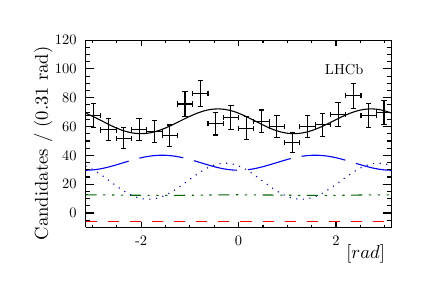
\begin{tikzpicture}
\pgfdeclareplotmark{cross} {
\pgfpathmoveto{\pgfpoint{-0.3\pgfplotmarksize}{\pgfplotmarksize}}
\pgfpathlineto{\pgfpoint{+0.3\pgfplotmarksize}{\pgfplotmarksize}}
\pgfpathlineto{\pgfpoint{+0.3\pgfplotmarksize}{0.3\pgfplotmarksize}}
\pgfpathlineto{\pgfpoint{+1\pgfplotmarksize}{0.3\pgfplotmarksize}}
\pgfpathlineto{\pgfpoint{+1\pgfplotmarksize}{-0.3\pgfplotmarksize}}
\pgfpathlineto{\pgfpoint{+0.3\pgfplotmarksize}{-0.3\pgfplotmarksize}}
\pgfpathlineto{\pgfpoint{+0.3\pgfplotmarksize}{-1.\pgfplotmarksize}}
\pgfpathlineto{\pgfpoint{-0.3\pgfplotmarksize}{-1.\pgfplotmarksize}}
\pgfpathlineto{\pgfpoint{-0.3\pgfplotmarksize}{-0.3\pgfplotmarksize}}
\pgfpathlineto{\pgfpoint{-1.\pgfplotmarksize}{-0.3\pgfplotmarksize}}
\pgfpathlineto{\pgfpoint{-1.\pgfplotmarksize}{0.3\pgfplotmarksize}}
\pgfpathlineto{\pgfpoint{-0.3\pgfplotmarksize}{0.3\pgfplotmarksize}}
\pgfpathclose
\pgfusepathqstroke
}
\pgfdeclareplotmark{cross*} {
\pgfpathmoveto{\pgfpoint{-0.3\pgfplotmarksize}{\pgfplotmarksize}}
\pgfpathlineto{\pgfpoint{+0.3\pgfplotmarksize}{\pgfplotmarksize}}
\pgfpathlineto{\pgfpoint{+0.3\pgfplotmarksize}{0.3\pgfplotmarksize}}
\pgfpathlineto{\pgfpoint{+1\pgfplotmarksize}{0.3\pgfplotmarksize}}
\pgfpathlineto{\pgfpoint{+1\pgfplotmarksize}{-0.3\pgfplotmarksize}}
\pgfpathlineto{\pgfpoint{+0.3\pgfplotmarksize}{-0.3\pgfplotmarksize}}
\pgfpathlineto{\pgfpoint{+0.3\pgfplotmarksize}{-1.\pgfplotmarksize}}
\pgfpathlineto{\pgfpoint{-0.3\pgfplotmarksize}{-1.\pgfplotmarksize}}
\pgfpathlineto{\pgfpoint{-0.3\pgfplotmarksize}{-0.3\pgfplotmarksize}}
\pgfpathlineto{\pgfpoint{-1.\pgfplotmarksize}{-0.3\pgfplotmarksize}}
\pgfpathlineto{\pgfpoint{-1.\pgfplotmarksize}{0.3\pgfplotmarksize}}
\pgfpathlineto{\pgfpoint{-0.3\pgfplotmarksize}{0.3\pgfplotmarksize}}
\pgfpathclose
\pgfusepathqfillstroke
}
\pgfdeclareplotmark{newstar} {
\pgfpathmoveto{\pgfqpoint{0pt}{\pgfplotmarksize}}
\pgfpathlineto{\pgfqpointpolar{44}{0.5\pgfplotmarksize}}
\pgfpathlineto{\pgfqpointpolar{18}{\pgfplotmarksize}}
\pgfpathlineto{\pgfqpointpolar{-20}{0.5\pgfplotmarksize}}
\pgfpathlineto{\pgfqpointpolar{-54}{\pgfplotmarksize}}
\pgfpathlineto{\pgfqpointpolar{-90}{0.5\pgfplotmarksize}}
\pgfpathlineto{\pgfqpointpolar{234}{\pgfplotmarksize}}
\pgfpathlineto{\pgfqpointpolar{198}{0.5\pgfplotmarksize}}
\pgfpathlineto{\pgfqpointpolar{162}{\pgfplotmarksize}}
\pgfpathlineto{\pgfqpointpolar{134}{0.5\pgfplotmarksize}}
\pgfpathclose
\pgfusepathqstroke
}
\pgfdeclareplotmark{newstar*} {
\pgfpathmoveto{\pgfqpoint{0pt}{\pgfplotmarksize}}
\pgfpathlineto{\pgfqpointpolar{44}{0.5\pgfplotmarksize}}
\pgfpathlineto{\pgfqpointpolar{18}{\pgfplotmarksize}}
\pgfpathlineto{\pgfqpointpolar{-20}{0.5\pgfplotmarksize}}
\pgfpathlineto{\pgfqpointpolar{-54}{\pgfplotmarksize}}
\pgfpathlineto{\pgfqpointpolar{-90}{0.5\pgfplotmarksize}}
\pgfpathlineto{\pgfqpointpolar{234}{\pgfplotmarksize}}
\pgfpathlineto{\pgfqpointpolar{198}{0.5\pgfplotmarksize}}
\pgfpathlineto{\pgfqpointpolar{162}{\pgfplotmarksize}}
\pgfpathlineto{\pgfqpointpolar{134}{0.5\pgfplotmarksize}}
\pgfpathclose
\pgfusepathqfillstroke
}
\definecolor{c}{rgb}{1,1,1};
\draw [color=c, fill=c] (0.1,0.0627517) rectangle (4.9,3.07483);
\draw [color=c, fill=c] (0.772,0.544685) rectangle (4.66,2.92423);
\definecolor{c}{rgb}{0,0,0};
\draw [c] (0.772,0.544685) -- (0.772,2.92423) -- (4.66,2.92423) -- (4.66,0.544685) -- (0.772,0.544685);
\definecolor{c}{rgb}{1,1,1};
\draw [color=c, fill=c] (0.772,0.544685) rectangle (4.66,2.92423);
\definecolor{c}{rgb}{0,0,0};
\draw [c] (0.772,0.544685) -- (0.772,2.92423) -- (4.66,2.92423) -- (4.66,0.544685) -- (0.772,0.544685);
\draw [c,line width=0.4] (0.772,0.544685) -- (4.66,0.544685);
\draw [anchor= east] (4.66,0.207332) node[scale=0.672711, rotate=0]{$\phihel [\text{rad}]$};
\draw [c,line width=0.4] (1.47841,0.617878) -- (1.47841,0.544685);
\draw [c,line width=0.4] (1.78781,0.581281) -- (1.78781,0.544685);
\draw [c,line width=0.4] (2.09721,0.581281) -- (2.09721,0.544685);
\draw [c,line width=0.4] (2.4066,0.581281) -- (2.4066,0.544685);
\draw [c,line width=0.4] (2.716,0.617878) -- (2.716,0.544685);
\draw [c,line width=0.4] (3.0254,0.581281) -- (3.0254,0.544685);
\draw [c,line width=0.4] (3.33479,0.581281) -- (3.33479,0.544685);
\draw [c,line width=0.4] (3.64419,0.581281) -- (3.64419,0.544685);
\draw [c,line width=0.4] (3.95359,0.617878) -- (3.95359,0.544685);
\draw [c,line width=0.4] (1.47841,0.617878) -- (1.47841,0.544685);
\draw [c,line width=0.4] (1.16901,0.581281) -- (1.16901,0.544685);
\draw [c,line width=0.4] (0.859617,0.581281) -- (0.859617,0.544685);
\draw [c,line width=0.4] (3.95359,0.617878) -- (3.95359,0.544685);
\draw [c,line width=0.4] (4.26299,0.581281) -- (4.26299,0.544685);
\draw [c,line width=0.4] (4.57238,0.581281) -- (4.57238,0.544685);
\draw [anchor=base] (1.47841,0.321791) node[scale=0.52322, rotate=0]{-2};
\draw [anchor=base] (2.716,0.321791) node[scale=0.52322, rotate=0]{0};
\draw [anchor=base] (3.95359,0.321791) node[scale=0.52322, rotate=0]{2};
\draw [c,line width=0.4] (0.772,2.92423) -- (4.66,2.92423);
\draw [c,line width=0.4] (1.47841,2.85103) -- (1.47841,2.92423);
\draw [c,line width=0.4] (1.78781,2.88763) -- (1.78781,2.92423);
\draw [c,line width=0.4] (2.09721,2.88763) -- (2.09721,2.92423);
\draw [c,line width=0.4] (2.4066,2.88763) -- (2.4066,2.92423);
\draw [c,line width=0.4] (2.716,2.85103) -- (2.716,2.92423);
\draw [c,line width=0.4] (3.0254,2.88763) -- (3.0254,2.92423);
\draw [c,line width=0.4] (3.33479,2.88763) -- (3.33479,2.92423);
\draw [c,line width=0.4] (3.64419,2.88763) -- (3.64419,2.92423);
\draw [c,line width=0.4] (3.95359,2.85103) -- (3.95359,2.92423);
\draw [c,line width=0.4] (1.47841,2.85103) -- (1.47841,2.92423);
\draw [c,line width=0.4] (1.16901,2.88763) -- (1.16901,2.92423);
\draw [c,line width=0.4] (0.859617,2.88763) -- (0.859617,2.92423);
\draw [c,line width=0.4] (3.95359,2.85103) -- (3.95359,2.92423);
\draw [c,line width=0.4] (4.26299,2.88763) -- (4.26299,2.92423);
\draw [c,line width=0.4] (4.57238,2.88763) -- (4.57238,2.92423);
\draw [c,line width=0.4] (0.772,0.544685) -- (0.772,2.92423);
\draw [anchor= east] (0.2344,2.92423) node[scale=0.672711, rotate=90]{Candidates / (0.31 rad)};
\draw [c,line width=0.4] (0.88576,0.727726) -- (0.772,0.727726);
\draw [c,line width=0.4] (0.82888,0.819247) -- (0.772,0.819247);
\draw [c,line width=0.4] (0.82888,0.910768) -- (0.772,0.910768);
\draw [c,line width=0.4] (0.82888,1.00229) -- (0.772,1.00229);
\draw [c,line width=0.4] (0.88576,1.09381) -- (0.772,1.09381);
\draw [c,line width=0.4] (0.82888,1.18533) -- (0.772,1.18533);
\draw [c,line width=0.4] (0.82888,1.27685) -- (0.772,1.27685);
\draw [c,line width=0.4] (0.82888,1.36837) -- (0.772,1.36837);
\draw [c,line width=0.4] (0.88576,1.45989) -- (0.772,1.45989);
\draw [c,line width=0.4] (0.82888,1.55141) -- (0.772,1.55141);
\draw [c,line width=0.4] (0.82888,1.64294) -- (0.772,1.64294);
\draw [c,line width=0.4] (0.82888,1.73446) -- (0.772,1.73446);
\draw [c,line width=0.4] (0.88576,1.82598) -- (0.772,1.82598);
\draw [c,line width=0.4] (0.82888,1.9175) -- (0.772,1.9175);
\draw [c,line width=0.4] (0.82888,2.00902) -- (0.772,2.00902);
\draw [c,line width=0.4] (0.82888,2.10054) -- (0.772,2.10054);
\draw [c,line width=0.4] (0.88576,2.19206) -- (0.772,2.19206);
\draw [c,line width=0.4] (0.82888,2.28358) -- (0.772,2.28358);
\draw [c,line width=0.4] (0.82888,2.3751) -- (0.772,2.3751);
\draw [c,line width=0.4] (0.82888,2.46662) -- (0.772,2.46662);
\draw [c,line width=0.4] (0.88576,2.55814) -- (0.772,2.55814);
\draw [c,line width=0.4] (0.82888,2.64967) -- (0.772,2.64967);
\draw [c,line width=0.4] (0.82888,2.74119) -- (0.772,2.74119);
\draw [c,line width=0.4] (0.82888,2.83271) -- (0.772,2.83271);
\draw [c,line width=0.4] (0.88576,2.92423) -- (0.772,2.92423);
\draw [c,line width=0.4] (0.88576,0.727726) -- (0.772,0.727726);
\draw [c,line width=0.4] (0.82888,0.636205) -- (0.772,0.636205);
\draw [c,line width=0.4] (0.82888,0.544685) -- (0.772,0.544685);
\draw [anchor= east] (0.724,0.727726) node[scale=0.52322, rotate=0]{0};
\draw [anchor= east] (0.724,1.09381) node[scale=0.52322, rotate=0]{20};
\draw [anchor= east] (0.724,1.45989) node[scale=0.52322, rotate=0]{40};
\draw [anchor= east] (0.724,1.82598) node[scale=0.52322, rotate=0]{60};
\draw [anchor= east] (0.724,2.19206) node[scale=0.52322, rotate=0]{80};
\draw [anchor= east] (0.724,2.55814) node[scale=0.52322, rotate=0]{100};
\draw [anchor= east] (0.724,2.92423) node[scale=0.52322, rotate=0]{120};
\draw [c,line width=0.4] (4.66,0.544685) -- (4.66,2.92423);
\draw [c,line width=0.4] (4.54624,0.727726) -- (4.66,0.727726);
\draw [c,line width=0.4] (4.60312,0.819247) -- (4.66,0.819247);
\draw [c,line width=0.4] (4.60312,0.910768) -- (4.66,0.910768);
\draw [c,line width=0.4] (4.60312,1.00229) -- (4.66,1.00229);
\draw [c,line width=0.4] (4.54624,1.09381) -- (4.66,1.09381);
\draw [c,line width=0.4] (4.60312,1.18533) -- (4.66,1.18533);
\draw [c,line width=0.4] (4.60312,1.27685) -- (4.66,1.27685);
\draw [c,line width=0.4] (4.60312,1.36837) -- (4.66,1.36837);
\draw [c,line width=0.4] (4.54624,1.45989) -- (4.66,1.45989);
\draw [c,line width=0.4] (4.60312,1.55141) -- (4.66,1.55141);
\draw [c,line width=0.4] (4.60312,1.64294) -- (4.66,1.64294);
\draw [c,line width=0.4] (4.60312,1.73446) -- (4.66,1.73446);
\draw [c,line width=0.4] (4.54624,1.82598) -- (4.66,1.82598);
\draw [c,line width=0.4] (4.60312,1.9175) -- (4.66,1.9175);
\draw [c,line width=0.4] (4.60312,2.00902) -- (4.66,2.00902);
\draw [c,line width=0.4] (4.60312,2.10054) -- (4.66,2.10054);
\draw [c,line width=0.4] (4.54624,2.19206) -- (4.66,2.19206);
\draw [c,line width=0.4] (4.60312,2.28358) -- (4.66,2.28358);
\draw [c,line width=0.4] (4.60312,2.3751) -- (4.66,2.3751);
\draw [c,line width=0.4] (4.60312,2.46662) -- (4.66,2.46662);
\draw [c,line width=0.4] (4.54624,2.55814) -- (4.66,2.55814);
\draw [c,line width=0.4] (4.60312,2.64967) -- (4.66,2.64967);
\draw [c,line width=0.4] (4.60312,2.74119) -- (4.66,2.74119);
\draw [c,line width=0.4] (4.60312,2.83271) -- (4.66,2.83271);
\draw [c,line width=0.4] (4.54624,2.92423) -- (4.66,2.92423);
\draw [c,line width=0.4] (4.54624,0.727726) -- (4.66,0.727726);
\draw [c,line width=0.4] (4.60312,0.636205) -- (4.66,0.636205);
\draw [c,line width=0.4] (4.60312,0.544685) -- (4.66,0.544685);
\draw [c] (0.8692,1.96341) -- (0.772,1.96341);
\draw [c] (0.772,1.92985) -- (0.772,1.99697);
\draw [c] (0.8692,1.96341) -- (0.9664,1.96341);
\draw [c] (0.9664,1.92985) -- (0.9664,1.99697);
\draw [c] (0.8692,1.96341) -- (0.8692,2.117);
\draw [c] (0.835643,2.117) -- (0.902757,2.117);
\draw [c] (0.8692,1.96341) -- (0.8692,1.80982);
\draw [c] (0.835643,1.80982) -- (0.902757,1.80982);
\draw [c] (1.0636,1.78392) -- (0.9664,1.78392);
\draw [c] (0.9664,1.75037) -- (0.9664,1.81748);
\draw [c] (1.0636,1.78392) -- (1.1608,1.78392);
\draw [c] (1.1608,1.75037) -- (1.1608,1.81748);
\draw [c] (1.0636,1.78392) -- (1.0636,1.92382);
\draw [c] (1.03004,1.92382) -- (1.09716,1.92382);
\draw [c] (1.0636,1.78392) -- (1.0636,1.64403);
\draw [c] (1.03004,1.64403) -- (1.09716,1.64403);
\draw [c] (1.258,1.67889) -- (1.1608,1.67889);
\draw [c] (1.1608,1.64533) -- (1.1608,1.71245);
\draw [c] (1.258,1.67889) -- (1.3552,1.67889);
\draw [c] (1.3552,1.64533) -- (1.3552,1.71245);
\draw [c] (1.258,1.67889) -- (1.258,1.81405);
\draw [c] (1.22444,1.81405) -- (1.29156,1.81405);
\draw [c] (1.258,1.67889) -- (1.258,1.54373);
\draw [c] (1.22444,1.54373) -- (1.29156,1.54373);
\draw [c] (1.4524,1.78673) -- (1.3552,1.78673);
\draw [c] (1.3552,1.75318) -- (1.3552,1.82029);
\draw [c] (1.4524,1.78673) -- (1.5496,1.78673);
\draw [c] (1.5496,1.75318) -- (1.5496,1.82029);
\draw [c] (1.4524,1.78673) -- (1.4524,1.92658);
\draw [c] (1.41884,1.92658) -- (1.48596,1.92658);
\draw [c] (1.4524,1.78673) -- (1.4524,1.64688);
\draw [c] (1.41884,1.64688) -- (1.48596,1.64688);
\draw [c] (1.6468,1.76304) -- (1.5496,1.76304);
\draw [c] (1.5496,1.72948) -- (1.5496,1.7966);
\draw [c] (1.6468,1.76304) -- (1.744,1.76304);
\draw [c] (1.744,1.72948) -- (1.744,1.7966);
\draw [c] (1.6468,1.76304) -- (1.6468,1.90055);
\draw [c] (1.61324,1.90055) -- (1.68036,1.90055);
\draw [c] (1.6468,1.76304) -- (1.6468,1.62553);
\draw [c] (1.61324,1.62553) -- (1.68036,1.62553);
\draw [c] (1.8412,1.70951) -- (1.744,1.70951);
\draw [c] (1.744,1.67595) -- (1.744,1.74306);
\draw [c] (1.8412,1.70951) -- (1.9384,1.70951);
\draw [c] (1.9384,1.67595) -- (1.9384,1.74306);
\draw [c] (1.8412,1.70951) -- (1.8412,1.84596);
\draw [c] (1.80764,1.84596) -- (1.87476,1.84596);
\draw [c] (1.8412,1.70951) -- (1.8412,1.57305);
\draw [c] (1.80764,1.57305) -- (1.87476,1.57305);
\draw [c] (2.0356,2.11235) -- (1.9384,2.11235);
\draw [c] (1.9384,2.07879) -- (1.9384,2.14591);
\draw [c] (2.0356,2.11235) -- (2.1328,2.11235);
\draw [c] (2.1328,2.07879) -- (2.1328,2.14591);
\draw [c] (2.0356,2.11235) -- (2.0356,2.26707);
\draw [c] (2.00204,2.26707) -- (2.06916,2.26707);
\draw [c] (2.0356,2.11235) -- (2.0356,1.95764);
\draw [c] (2.00204,1.95764) -- (2.06916,1.95764);
\draw [c] (2.23,2.24394) -- (2.1328,2.24394);
\draw [c] (2.1328,2.21038) -- (2.1328,2.2775);
\draw [c] (2.23,2.24394) -- (2.3272,2.24394);
\draw [c] (2.3272,2.21038) -- (2.3272,2.2775);
\draw [c] (2.23,2.24394) -- (2.23,2.40814);
\draw [c] (2.19644,2.40814) -- (2.26356,2.40814);
\draw [c] (2.23,2.24394) -- (2.23,2.07974);
\draw [c] (2.19644,2.07974) -- (2.26356,2.07974);
\draw [c] (2.4244,1.86354) -- (2.3272,1.86354);
\draw [c] (2.3272,1.82999) -- (2.3272,1.8971);
\draw [c] (2.4244,1.86354) -- (2.5216,1.86354);
\draw [c] (2.5216,1.82999) -- (2.5216,1.8971);
\draw [c] (2.4244,1.86354) -- (2.4244,2.00843);
\draw [c] (2.39084,2.00843) -- (2.45796,2.00843);
\draw [c] (2.4244,1.86354) -- (2.4244,1.71866);
\draw [c] (2.39084,1.71866) -- (2.45796,1.71866);
\draw [c] (2.6188,1.94512) -- (2.5216,1.94512);
\draw [c] (2.5216,1.91156) -- (2.5216,1.97867);
\draw [c] (2.6188,1.94512) -- (2.716,1.94512);
\draw [c] (2.716,1.91156) -- (2.716,1.97867);
\draw [c] (2.6188,1.94512) -- (2.6188,2.09682);
\draw [c] (2.58524,2.09682) -- (2.65236,2.09682);
\draw [c] (2.6188,1.94512) -- (2.6188,1.79341);
\draw [c] (2.58524,1.79341) -- (2.65236,1.79341);
\draw [c] (2.8132,1.80577) -- (2.716,1.80577);
\draw [c] (2.716,1.77221) -- (2.716,1.83932);
\draw [c] (2.8132,1.80577) -- (2.9104,1.80577);
\draw [c] (2.9104,1.77221) -- (2.9104,1.83932);
\draw [c] (2.8132,1.80577) -- (2.8132,1.94954);
\draw [c] (2.77964,1.94954) -- (2.84676,1.94954);
\draw [c] (2.8132,1.80577) -- (2.8132,1.66199);
\draw [c] (2.77964,1.66199) -- (2.84676,1.66199);
\draw [c] (3.0076,1.89231) -- (2.9104,1.89231);
\draw [c] (2.9104,1.85875) -- (2.9104,1.92586);
\draw [c] (3.0076,1.89231) -- (3.1048,1.89231);
\draw [c] (3.1048,1.85875) -- (3.1048,1.92586);
\draw [c] (3.0076,1.89231) -- (3.0076,2.03691);
\draw [c] (2.97404,2.03691) -- (3.04116,2.03691);
\draw [c] (3.0076,1.89231) -- (3.0076,1.74771);
\draw [c] (2.97404,1.74771) -- (3.04116,1.74771);
\draw [c] (3.202,1.83062) -- (3.1048,1.83062);
\draw [c] (3.1048,1.79706) -- (3.1048,1.86418);
\draw [c] (3.202,1.83062) -- (3.2992,1.83062);
\draw [c] (3.2992,1.79706) -- (3.2992,1.86418);
\draw [c] (3.202,1.83062) -- (3.202,1.97006);
\draw [c] (3.16844,1.97006) -- (3.23556,1.97006);
\draw [c] (3.202,1.83062) -- (3.202,1.69118);
\draw [c] (3.16844,1.69118) -- (3.23556,1.69118);
\draw [c] (3.3964,1.62415) -- (3.2992,1.62415);
\draw [c] (3.2992,1.5906) -- (3.2992,1.65771);
\draw [c] (3.3964,1.62415) -- (3.4936,1.62415);
\draw [c] (3.4936,1.5906) -- (3.4936,1.65771);
\draw [c] (3.3964,1.62415) -- (3.3964,1.75548);
\draw [c] (3.36284,1.75548) -- (3.42996,1.75548);
\draw [c] (3.3964,1.62415) -- (3.3964,1.49283);
\draw [c] (3.36284,1.49283) -- (3.42996,1.49283);
\draw [c] (3.5908,1.8249) -- (3.4936,1.8249);
\draw [c] (3.4936,1.79135) -- (3.4936,1.85846);
\draw [c] (3.5908,1.8249) -- (3.688,1.8249);
\draw [c] (3.688,1.79135) -- (3.688,1.85846);
\draw [c] (3.5908,1.8249) -- (3.5908,1.96821);
\draw [c] (3.55724,1.96821) -- (3.62436,1.96821);
\draw [c] (3.5908,1.8249) -- (3.5908,1.6816);
\draw [c] (3.55724,1.6816) -- (3.62436,1.6816);
\draw [c] (3.7852,1.84784) -- (3.688,1.84784);
\draw [c] (3.688,1.81429) -- (3.688,1.8814);
\draw [c] (3.7852,1.84784) -- (3.8824,1.84784);
\draw [c] (3.8824,1.81429) -- (3.8824,1.8814);
\draw [c] (3.7852,1.84784) -- (3.7852,1.99152);
\draw [c] (3.75164,1.99152) -- (3.81876,1.99152);
\draw [c] (3.7852,1.84784) -- (3.7852,1.70417);
\draw [c] (3.75164,1.70417) -- (3.81876,1.70417);
\draw [c] (3.9796,1.97861) -- (3.8824,1.97861);
\draw [c] (3.8824,1.94505) -- (3.8824,2.01217);
\draw [c] (3.9796,1.97861) -- (4.0768,1.97861);
\draw [c] (4.0768,1.94505) -- (4.0768,2.01217);
\draw [c] (3.9796,1.97861) -- (3.9796,2.12764);
\draw [c] (3.94604,2.12764) -- (4.01316,2.12764);
\draw [c] (3.9796,1.97861) -- (3.9796,1.82958);
\draw [c] (3.94604,1.82958) -- (4.01316,1.82958);
\draw [c] (4.174,2.21803) -- (4.0768,2.21803);
\draw [c] (4.0768,2.18447) -- (4.0768,2.25158);
\draw [c] (4.174,2.21803) -- (4.2712,2.21803);
\draw [c] (4.2712,2.18447) -- (4.2712,2.25158);
\draw [c] (4.174,2.21803) -- (4.174,2.37723);
\draw [c] (4.14044,2.37723) -- (4.20756,2.37723);
\draw [c] (4.174,2.21803) -- (4.174,2.05882);
\draw [c] (4.14044,2.05882) -- (4.20756,2.05882);
\draw [c] (4.3684,1.96615) -- (4.2712,1.96615);
\draw [c] (4.2712,1.93259) -- (4.2712,1.9997);
\draw [c] (4.3684,1.96615) -- (4.4656,1.96615);
\draw [c] (4.4656,1.93259) -- (4.4656,1.9997);
\draw [c] (4.3684,1.96615) -- (4.3684,2.11572);
\draw [c] (4.33484,2.11572) -- (4.40196,2.11572);
\draw [c] (4.3684,1.96615) -- (4.3684,1.81658);
\draw [c] (4.33484,1.81658) -- (4.40196,1.81658);
\draw [c] (4.5628,2.00459) -- (4.4656,2.00459);
\draw [c] (4.4656,1.97103) -- (4.4656,2.03814);
\draw [c] (4.5628,2.00459) -- (4.66,2.00459);
\draw [c] (4.66,1.97103) -- (4.66,2.03814);
\draw [c] (4.5628,2.00459) -- (4.5628,2.15785);
\draw [c] (4.52924,2.15785) -- (4.59636,2.15785);
\draw [c] (4.5628,2.00459) -- (4.5628,1.85132);
\draw [c] (4.52924,1.85132) -- (4.59636,1.85132);
\foreach \P in
 {(0.8692,1.96341),(1.0636,1.78392),(1.258,1.67889),(1.4524,1.78673),(1.6468,1.76304),(1.8412,1.70951),(2.0356,2.11235),(2.23,2.24394),(2.4244,1.86354),(2.6188,1.94512),(2.8132,1.80577),(3.0076,1.89231),(3.202,1.83062),(3.3964,1.62415),(3.5908,1.8249
),(3.7852,1.84784),(3.9796,1.97861),(4.174,2.21803),(4.3684,1.96615),(4.5628,2.00459)}{\draw[mark options={color=c,fill=c},mark size=1.201201pt,mark=] plot coordinates {\P};}
\definecolor{c}{rgb}{1,0,0};
\draw [c,dash pattern=on 4pt off 4pt] (0.772,0.622545) -- (0.772,0.622545);
\draw [c,dash pattern=on 4pt off 4pt] (0.772,0.622545) -- (0.9664,0.622545) -- (1.1608,0.622545) -- (1.3552,0.622545) -- (1.5496,0.622545) -- (1.744,0.622545) -- (1.9384,0.622545) -- (2.1328,0.622545) -- (2.3272,0.622545) -- (2.5216,0.622545) --
 (2.716,0.622545) -- (2.9104,0.622545) -- (3.1048,0.622545) -- (3.2992,0.622545) -- (3.4936,0.622545) -- (3.688,0.622545) -- (3.8824,0.622545) -- (4.0768,0.622545) -- (4.2712,0.622545) -- (4.4656,0.622545) -- (4.66,0.622545) -- (4.66,0.622545) --
 (4.66,0.622545);
\definecolor{c}{rgb}{0,0.4,0};
\draw [c,dash pattern=on 4pt off 2.4pt on 0.8pt off 2.4pt on 0.8pt off 2.4pt on 0.8pt off 2.4pt] (0.772,0.959345) -- (0.772,0.959345);
\draw [c,dash pattern=on 4pt off 2.4pt on 0.8pt off 2.4pt on 0.8pt off 2.4pt on 0.8pt off 2.4pt] (0.772,0.959345) -- (0.7963,0.959333) -- (0.8206,0.959297) -- (0.8449,0.959236) -- (0.8692,0.959152) -- (0.8935,0.959045) -- (0.9178,0.958916) --
 (0.9421,0.958765) -- (0.9664,0.958593) -- (0.9907,0.958401) -- (1.015,0.958191) -- (1.0393,0.957964) -- (1.0636,0.957721) -- (1.1122,0.957194) -- (1.1608,0.956623) -- (1.3552,0.954188) -- (1.4038,0.953617) -- (1.4524,0.953089) -- (1.4767,0.952847)
 -- (1.501,0.952619) -- (1.5253,0.952409) -- (1.5496,0.952218) -- (1.5739,0.952046) -- (1.5982,0.951895) -- (1.6225,0.951765) -- (1.6468,0.951658) -- (1.6711,0.951574) -- (1.6954,0.951514) -- (1.7197,0.951478) -- (1.744,0.951465) -- (1.7683,0.951478)
 -- (1.7926,0.951514) -- (1.8169,0.951574) -- (1.8412,0.951658) -- (1.8655,0.951765) -- (1.8898,0.951895) -- (1.9141,0.952046) -- (1.9384,0.952218) -- (1.9627,0.952409) -- (1.987,0.952619) -- (2.0113,0.952847) -- (2.0356,0.953089) --
 (2.0842,0.953617) -- (2.1328,0.954188) -- (2.3272,0.956623) -- (2.3758,0.957194) -- (2.4244,0.957721) -- (2.4487,0.957964) -- (2.473,0.958191) -- (2.4973,0.958401) -- (2.5216,0.958593) -- (2.5459,0.958765) -- (2.5702,0.958916) -- (2.5945,0.959045)
 -- (2.6188,0.959152) -- (2.6431,0.959236) -- (2.6674,0.959297) -- (2.6917,0.959333) -- (2.716,0.959345) -- (2.7403,0.959333) -- (2.7646,0.959297) -- (2.7889,0.959236) -- (2.8132,0.959152) -- (2.8375,0.959045) -- (2.8618,0.958916) --
 (2.8861,0.958765) -- (2.9104,0.958593) -- (2.9347,0.958401) -- (2.959,0.958191) -- (2.9833,0.957964) -- (3.0076,0.957721) -- (3.0562,0.957194) -- (3.1048,0.956623) -- (3.2992,0.954188) -- (3.3478,0.953617) -- (3.3964,0.953089) -- (3.4207,0.952847)
 -- (3.445,0.952619) -- (3.4693,0.952409) -- (3.4936,0.952218) -- (3.5179,0.952046) -- (3.5422,0.951895) -- (3.5665,0.951765) -- (3.5908,0.951658) -- (3.6151,0.951574) -- (3.6394,0.951514) -- (3.6637,0.951478) -- (3.688,0.951465) -- (3.7123,0.951478)
 -- (3.7366,0.951514) -- (3.7609,0.951574) -- (3.7852,0.951658) -- (3.8095,0.951765) -- (3.8338,0.951895) -- (3.8581,0.952046) -- (3.8824,0.952218) -- (3.9067,0.952409) -- (3.931,0.952619) -- (3.9553,0.952847) -- (3.9796,0.953089) --
 (4.0282,0.953617) -- (4.0768,0.954188) -- (4.2712,0.956623) -- (4.3198,0.957194) -- (4.3684,0.957721) -- (4.3927,0.957964) -- (4.417,0.958191) -- (4.4413,0.958401) -- (4.4656,0.958593) -- (4.4899,0.958765) -- (4.5142,0.958916) -- (4.5385,0.959045)
 -- (4.5628,0.959152) -- (4.5871,0.959236) -- (4.6114,0.959297) -- (4.6357,0.959333) -- (4.66,0.959345) -- (4.66,0.959345) -- (4.66,0.959345);
\definecolor{c}{rgb}{0,0,1};
\draw [c,dotted] (0.772,1.32623) -- (0.772,1.32623);
\draw [c,dotted] (0.772,1.32623) -- (0.7963,1.31602) -- (0.8206,1.30463) -- (0.8449,1.29213) -- (0.8692,1.27862) -- (0.9178,1.24888) -- (0.9664,1.2162) -- (1.015,1.18143) -- (1.0636,1.14547) -- (1.1608,1.07364) -- (1.2094,1.03959) -- (1.258,1.00791)
 -- (1.3066,0.979361) -- (1.3309,0.966474) -- (1.3552,0.954615) -- (1.3795,0.943851) -- (1.4038,0.934242) -- (1.4281,0.925843) -- (1.4524,0.918698) -- (1.4767,0.912845) -- (1.501,0.908316) -- (1.5253,0.905132) -- (1.5496,0.903309) --
 (1.5739,0.902852) -- (1.5982,0.903762) -- (1.6225,0.90603) -- (1.6468,0.909639) -- (1.6711,0.914568) -- (1.6954,0.920785) -- (1.7197,0.928253) -- (1.744,0.936928) -- (1.7683,0.946759) -- (1.7926,0.957689) -- (1.8169,0.969655) -- (1.8412,0.982587) --
 (1.8898,1.01105) -- (1.9384,1.04242) -- (1.987,1.07598) -- (2.0356,1.11095) -- (2.1328,1.18177) -- (2.1814,1.21591) -- (2.23,1.24809) -- (2.2786,1.27748) -- (2.3029,1.2909) -- (2.3272,1.30334) -- (2.3515,1.31473) -- (2.3758,1.32498) --
 (2.4001,1.33404) -- (2.4244,1.34183) -- (2.4487,1.34831) -- (2.473,1.35343) -- (2.4973,1.35714) -- (2.5216,1.35943) -- (2.5459,1.36028) -- (2.5702,1.35967) -- (2.5945,1.35761) -- (2.6188,1.35411) -- (2.6431,1.34918) -- (2.6674,1.34287) --
 (2.6917,1.3352) -- (2.716,1.32623) -- (2.7403,1.31602) -- (2.7646,1.30463) -- (2.7889,1.29213) -- (2.8132,1.27862) -- (2.8618,1.24888) -- (2.9104,1.2162) -- (2.959,1.18143) -- (3.0076,1.14547) -- (3.1048,1.07364) -- (3.1534,1.03959) --
 (3.202,1.00791) -- (3.2506,0.979361) -- (3.2749,0.966474) -- (3.2992,0.954615) -- (3.3235,0.943851) -- (3.3478,0.934242) -- (3.3721,0.925843) -- (3.3964,0.918698) -- (3.4207,0.912845) -- (3.445,0.908316) -- (3.4693,0.905132) -- (3.4936,0.903309) --
 (3.5179,0.902852) -- (3.5422,0.903762) -- (3.5665,0.90603) -- (3.5908,0.909639) -- (3.6151,0.914568) -- (3.6394,0.920785) -- (3.6637,0.928253) -- (3.688,0.936928) -- (3.7123,0.946759) -- (3.7366,0.957689) -- (3.7609,0.969655) -- (3.7852,0.982587) --
 (3.8338,1.01105) -- (3.8824,1.04242) -- (3.931,1.07598) -- (3.9796,1.11095) -- (4.0768,1.18177) -- (4.1254,1.21591) -- (4.174,1.24809) -- (4.2226,1.27748) -- (4.2469,1.2909) -- (4.2712,1.30334) -- (4.2955,1.31473) -- (4.3198,1.32498) --
 (4.3441,1.33404) -- (4.3684,1.34183) -- (4.3927,1.34831) -- (4.417,1.35343) -- (4.4413,1.35714) -- (4.4656,1.35943) -- (4.4899,1.36028) -- (4.5142,1.35967) -- (4.5385,1.35761) -- (4.5628,1.35411) -- (4.5871,1.34918) -- (4.6114,1.34287) --
 (4.6357,1.3352) -- (4.66,1.32623) -- (4.66,1.32623) -- (4.66,1.32623);
\draw [c,dash pattern=on 16pt off 4pt] (0.772,1.27147) -- (0.772,1.27147);
\draw [c,dash pattern=on 16pt off 4pt] (0.772,1.27147) -- (0.7963,1.27177) -- (0.8206,1.27269) -- (0.8449,1.2742) -- (0.8692,1.27631) -- (0.8935,1.279) -- (0.9178,1.28224) -- (0.9421,1.28602) -- (0.9664,1.29031) -- (0.9907,1.29508) -- (1.015,1.30031)
 -- (1.0636,1.31196) -- (1.1122,1.32496) -- (1.1608,1.33897) -- (1.3552,1.3978) -- (1.4038,1.41139) -- (1.4524,1.42385) -- (1.4767,1.42958) -- (1.501,1.43491) -- (1.5253,1.43984) -- (1.5496,1.44432) -- (1.5739,1.44833) -- (1.5982,1.45185) --
 (1.6225,1.45487) -- (1.6468,1.45736) -- (1.6711,1.45931) -- (1.6954,1.46071) -- (1.7197,1.46155) -- (1.744,1.46183) -- (1.7683,1.46155) -- (1.7926,1.46071) -- (1.8169,1.45931) -- (1.8412,1.45736) -- (1.8655,1.45487) -- (1.8898,1.45185) --
 (1.9141,1.44833) -- (1.9384,1.44432) -- (1.9627,1.43984) -- (1.987,1.43491) -- (2.0113,1.42958) -- (2.0356,1.42385) -- (2.0842,1.41139) -- (2.1328,1.3978) -- (2.3272,1.33897) -- (2.3758,1.32496) -- (2.4244,1.31196) -- (2.473,1.30031) --
 (2.4973,1.29508) -- (2.5216,1.29031) -- (2.5459,1.28602) -- (2.5702,1.28224) -- (2.5945,1.279) -- (2.6188,1.27631) -- (2.6431,1.2742) -- (2.6674,1.27269) -- (2.6917,1.27177) -- (2.716,1.27147) -- (2.7403,1.27177) -- (2.7646,1.27269) --
 (2.7889,1.2742) -- (2.8132,1.27631) -- (2.8375,1.279) -- (2.8618,1.28224) -- (2.8861,1.28602) -- (2.9104,1.29031) -- (2.9347,1.29508) -- (2.959,1.30031) -- (3.0076,1.31196) -- (3.0562,1.32496) -- (3.1048,1.33897) -- (3.2992,1.3978) --
 (3.3478,1.41139) -- (3.3964,1.42385) -- (3.4207,1.42958) -- (3.445,1.43491) -- (3.4693,1.43984) -- (3.4936,1.44432) -- (3.5179,1.44833) -- (3.5422,1.45185) -- (3.5665,1.45487) -- (3.5908,1.45736) -- (3.6151,1.45931) -- (3.6394,1.46071) --
 (3.6637,1.46155) -- (3.688,1.46183) -- (3.7123,1.46155) -- (3.7366,1.46071) -- (3.7609,1.45931) -- (3.7852,1.45736) -- (3.8095,1.45487) -- (3.8338,1.45185) -- (3.8581,1.44833) -- (3.8824,1.44432) -- (3.9067,1.43984) -- (3.931,1.43491) --
 (3.9553,1.42958) -- (3.9796,1.42385) -- (4.0282,1.41139) -- (4.0768,1.3978) -- (4.2712,1.33897) -- (4.3198,1.32496) -- (4.3684,1.31196) -- (4.417,1.30031) -- (4.4413,1.29508) -- (4.4656,1.29031) -- (4.4899,1.28602) -- (4.5142,1.28224) --
 (4.5385,1.279) -- (4.5628,1.27631) -- (4.5871,1.2742) -- (4.6114,1.27269) -- (4.6357,1.27177) -- (4.66,1.27147) -- (4.66,1.27147) -- (4.66,1.27147);
\definecolor{c}{rgb}{0,0,0};
\draw [c] (0.772,1.99565) -- (0.772,1.99565);
\draw [c] (0.772,1.99565) -- (0.8206,1.9754) -- (0.8692,1.95307) -- (0.9178,1.92922) -- (0.9664,1.90449) -- (1.0636,1.85491) -- (1.1122,1.83133) -- (1.1608,1.80935) -- (1.2094,1.78951) -- (1.2337,1.78054) -- (1.258,1.77228) -- (1.2823,1.76478) --
 (1.3066,1.75808) -- (1.3309,1.75222) -- (1.3552,1.74723) -- (1.3795,1.74313) -- (1.4038,1.73995) -- (1.4281,1.7377) -- (1.4524,1.73639) -- (1.4767,1.73603) -- (1.501,1.73662) -- (1.5253,1.73814) -- (1.5496,1.7406) -- (1.5739,1.74396) --
 (1.5982,1.74822) -- (1.6225,1.75333) -- (1.6468,1.75927) -- (1.6711,1.76601) -- (1.6954,1.7735) -- (1.7197,1.7817) -- (1.744,1.79056) -- (1.7926,1.81006) -- (1.8412,1.83154) -- (1.8898,1.8545) -- (1.9384,1.87841) -- (2.0356,1.92683) --
 (2.0842,1.95019) -- (2.1328,1.97223) -- (2.1814,1.9924) -- (2.2057,2.00162) -- (2.23,2.01019) -- (2.2543,2.01804) -- (2.2786,2.02514) -- (2.3029,2.03143) -- (2.3272,2.03686) -- (2.3515,2.0414) -- (2.3758,2.04502) -- (2.4001,2.0477) --
 (2.4244,2.0494) -- (2.4487,2.05013) -- (2.473,2.04986) -- (2.4973,2.0486) -- (2.5216,2.04635) -- (2.5459,2.04313) -- (2.5702,2.03895) -- (2.5945,2.03384) -- (2.6188,2.02784) -- (2.6431,2.02097) -- (2.6674,2.01328) -- (2.6917,2.00482) --
 (2.716,1.99565) -- (2.7646,1.9754) -- (2.8132,1.95307) -- (2.8618,1.92922) -- (2.9104,1.90449) -- (3.0076,1.85491) -- (3.0562,1.83133) -- (3.1048,1.80935) -- (3.1534,1.78951) -- (3.1777,1.78054) -- (3.202,1.77228) -- (3.2263,1.76478) --
 (3.2506,1.75808) -- (3.2749,1.75222) -- (3.2992,1.74723) -- (3.3235,1.74313) -- (3.3478,1.73995) -- (3.3721,1.7377) -- (3.3964,1.73639) -- (3.4207,1.73603) -- (3.445,1.73662) -- (3.4693,1.73814) -- (3.4936,1.7406) -- (3.5179,1.74396) --
 (3.5422,1.74822) -- (3.5665,1.75333) -- (3.5908,1.75927) -- (3.6151,1.76601) -- (3.6394,1.7735) -- (3.6637,1.7817) -- (3.688,1.79056) -- (3.7366,1.81006) -- (3.7852,1.83154) -- (3.8338,1.8545) -- (3.8824,1.87841) -- (3.9796,1.92683) --
 (4.0282,1.95019) -- (4.0768,1.97223) -- (4.1254,1.9924) -- (4.1497,2.00162) -- (4.174,2.01019) -- (4.1983,2.01804) -- (4.2226,2.02514) -- (4.2469,2.03143) -- (4.2712,2.03686) -- (4.2955,2.0414) -- (4.3198,2.04502) -- (4.3441,2.0477) --
 (4.3684,2.0494) -- (4.3927,2.05013) -- (4.417,2.04986) -- (4.4413,2.0486) -- (4.4656,2.04635) -- (4.4899,2.04313) -- (4.5142,2.03895) -- (4.5385,2.03384) -- (4.5628,2.02784) -- (4.5871,2.02097) -- (4.6114,2.01328) -- (4.6357,2.00482) --
 (4.66,1.99565) -- (4.66,1.99565) -- (4.66,1.99565);
\draw [c,line width=0.4] (0.772,0.544685) -- (4.66,0.544685);
\draw [c,line width=0.4] (1.47841,0.617878) -- (1.47841,0.544685);
\draw [c,line width=0.4] (1.78781,0.581281) -- (1.78781,0.544685);
\draw [c,line width=0.4] (2.09721,0.581281) -- (2.09721,0.544685);
\draw [c,line width=0.4] (2.4066,0.581281) -- (2.4066,0.544685);
\draw [c,line width=0.4] (2.716,0.617878) -- (2.716,0.544685);
\draw [c,line width=0.4] (3.0254,0.581281) -- (3.0254,0.544685);
\draw [c,line width=0.4] (3.33479,0.581281) -- (3.33479,0.544685);
\draw [c,line width=0.4] (3.64419,0.581281) -- (3.64419,0.544685);
\draw [c,line width=0.4] (3.95359,0.617878) -- (3.95359,0.544685);
\draw [c,line width=0.4] (1.47841,0.617878) -- (1.47841,0.544685);
\draw [c,line width=0.4] (1.16901,0.581281) -- (1.16901,0.544685);
\draw [c,line width=0.4] (0.859617,0.581281) -- (0.859617,0.544685);
\draw [c,line width=0.4] (3.95359,0.617878) -- (3.95359,0.544685);
\draw [c,line width=0.4] (4.26299,0.581281) -- (4.26299,0.544685);
\draw [c,line width=0.4] (4.57238,0.581281) -- (4.57238,0.544685);
\draw [c,line width=0.4] (0.772,2.92423) -- (4.66,2.92423);
\draw [c,line width=0.4] (1.47841,2.85103) -- (1.47841,2.92423);
\draw [c,line width=0.4] (1.78781,2.88763) -- (1.78781,2.92423);
\draw [c,line width=0.4] (2.09721,2.88763) -- (2.09721,2.92423);
\draw [c,line width=0.4] (2.4066,2.88763) -- (2.4066,2.92423);
\draw [c,line width=0.4] (2.716,2.85103) -- (2.716,2.92423);
\draw [c,line width=0.4] (3.0254,2.88763) -- (3.0254,2.92423);
\draw [c,line width=0.4] (3.33479,2.88763) -- (3.33479,2.92423);
\draw [c,line width=0.4] (3.64419,2.88763) -- (3.64419,2.92423);
\draw [c,line width=0.4] (3.95359,2.85103) -- (3.95359,2.92423);
\draw [c,line width=0.4] (1.47841,2.85103) -- (1.47841,2.92423);
\draw [c,line width=0.4] (1.16901,2.88763) -- (1.16901,2.92423);
\draw [c,line width=0.4] (0.859617,2.88763) -- (0.859617,2.92423);
\draw [c,line width=0.4] (3.95359,2.85103) -- (3.95359,2.92423);
\draw [c,line width=0.4] (4.26299,2.88763) -- (4.26299,2.92423);
\draw [c,line width=0.4] (4.57238,2.88763) -- (4.57238,2.92423);
\draw [c,line width=0.4] (0.772,0.544685) -- (0.772,2.92423);
\draw [c,line width=0.4] (0.88576,0.727726) -- (0.772,0.727726);
\draw [c,line width=0.4] (0.82888,0.819247) -- (0.772,0.819247);
\draw [c,line width=0.4] (0.82888,0.910768) -- (0.772,0.910768);
\draw [c,line width=0.4] (0.82888,1.00229) -- (0.772,1.00229);
\draw [c,line width=0.4] (0.88576,1.09381) -- (0.772,1.09381);
\draw [c,line width=0.4] (0.82888,1.18533) -- (0.772,1.18533);
\draw [c,line width=0.4] (0.82888,1.27685) -- (0.772,1.27685);
\draw [c,line width=0.4] (0.82888,1.36837) -- (0.772,1.36837);
\draw [c,line width=0.4] (0.88576,1.45989) -- (0.772,1.45989);
\draw [c,line width=0.4] (0.82888,1.55141) -- (0.772,1.55141);
\draw [c,line width=0.4] (0.82888,1.64294) -- (0.772,1.64294);
\draw [c,line width=0.4] (0.82888,1.73446) -- (0.772,1.73446);
\draw [c,line width=0.4] (0.88576,1.82598) -- (0.772,1.82598);
\draw [c,line width=0.4] (0.82888,1.9175) -- (0.772,1.9175);
\draw [c,line width=0.4] (0.82888,2.00902) -- (0.772,2.00902);
\draw [c,line width=0.4] (0.82888,2.10054) -- (0.772,2.10054);
\draw [c,line width=0.4] (0.88576,2.19206) -- (0.772,2.19206);
\draw [c,line width=0.4] (0.82888,2.28358) -- (0.772,2.28358);
\draw [c,line width=0.4] (0.82888,2.3751) -- (0.772,2.3751);
\draw [c,line width=0.4] (0.82888,2.46662) -- (0.772,2.46662);
\draw [c,line width=0.4] (0.88576,2.55814) -- (0.772,2.55814);
\draw [c,line width=0.4] (0.82888,2.64967) -- (0.772,2.64967);
\draw [c,line width=0.4] (0.82888,2.74119) -- (0.772,2.74119);
\draw [c,line width=0.4] (0.82888,2.83271) -- (0.772,2.83271);
\draw [c,line width=0.4] (0.88576,2.92423) -- (0.772,2.92423);
\draw [c,line width=0.4] (0.88576,0.727726) -- (0.772,0.727726);
\draw [c,line width=0.4] (0.82888,0.636205) -- (0.772,0.636205);
\draw [c,line width=0.4] (0.82888,0.544685) -- (0.772,0.544685);
\draw [c,line width=0.4] (4.66,0.544685) -- (4.66,2.92423);
\draw [c,line width=0.4] (4.54624,0.727726) -- (4.66,0.727726);
\draw [c,line width=0.4] (4.60312,0.819247) -- (4.66,0.819247);
\draw [c,line width=0.4] (4.60312,0.910768) -- (4.66,0.910768);
\draw [c,line width=0.4] (4.60312,1.00229) -- (4.66,1.00229);
\draw [c,line width=0.4] (4.54624,1.09381) -- (4.66,1.09381);
\draw [c,line width=0.4] (4.60312,1.18533) -- (4.66,1.18533);
\draw [c,line width=0.4] (4.60312,1.27685) -- (4.66,1.27685);
\draw [c,line width=0.4] (4.60312,1.36837) -- (4.66,1.36837);
\draw [c,line width=0.4] (4.54624,1.45989) -- (4.66,1.45989);
\draw [c,line width=0.4] (4.60312,1.55141) -- (4.66,1.55141);
\draw [c,line width=0.4] (4.60312,1.64294) -- (4.66,1.64294);
\draw [c,line width=0.4] (4.60312,1.73446) -- (4.66,1.73446);
\draw [c,line width=0.4] (4.54624,1.82598) -- (4.66,1.82598);
\draw [c,line width=0.4] (4.60312,1.9175) -- (4.66,1.9175);
\draw [c,line width=0.4] (4.60312,2.00902) -- (4.66,2.00902);
\draw [c,line width=0.4] (4.60312,2.10054) -- (4.66,2.10054);
\draw [c,line width=0.4] (4.54624,2.19206) -- (4.66,2.19206);
\draw [c,line width=0.4] (4.60312,2.28358) -- (4.66,2.28358);
\draw [c,line width=0.4] (4.60312,2.3751) -- (4.66,2.3751);
\draw [c,line width=0.4] (4.60312,2.46662) -- (4.66,2.46662);
\draw [c,line width=0.4] (4.54624,2.55814) -- (4.66,2.55814);
\draw [c,line width=0.4] (4.60312,2.64967) -- (4.66,2.64967);
\draw [c,line width=0.4] (4.60312,2.74119) -- (4.66,2.74119);
\draw [c,line width=0.4] (4.60312,2.83271) -- (4.66,2.83271);
\draw [c,line width=0.4] (4.54624,2.92423) -- (4.66,2.92423);
\draw [c,line width=0.4] (4.54624,0.727726) -- (4.66,0.727726);
\draw [c,line width=0.4] (4.60312,0.636205) -- (4.66,0.636205);
\draw [c,line width=0.4] (4.60312,0.544685) -- (4.66,0.544685);
\draw [anchor= west] (3.748,2.54772) node[scale=0.52322, rotate=0]{LHCb};
\end{tikzpicture}
}
  \end{subfigure}
  \caption{Het gefitte model (zwarte lijn) is op de \BsJpsiKst data (zwarte kruizen) afgebeeld.
          De verschillende componenten van het model die relevant zijn voor de \CP structuur zijn afgebeeld met gekleurde lijnen.}
  \label{app_nl_angular_plot_thetas}
\end{figure}

Uit de likelihood fit aan de data, met in acht name van \cite{Fleischer:1999zi,Faller:2008gt,DeBruyn:2014oga,DeBruyn-thesis},
volgt voor de bijdragen van de pingu\"in topologi\"en aan \phis:

% \begin{equation}
% \label{app_delta_phis_result}
%   \DeltaPhisPeng{0}         = 0.00 ^{+0.57}_{-0.80}, \;\;
%   \DeltaPhisPeng{\parallel} = 0.06 ^{+0.69}_{-0.92}, \;\;
%   \DeltaPhisPeng{\perp}     = 0.17 ^{+0.69}_{-0.92},
% \end{equation}

\begin{align}
\label{app_nl_delta_phis_result}
  \DeltaPhisPeng{0}         = 0.000 \; ^{+0.010}_{-0.014}, &\quad  \DeltaPhisPeng{\parallel} = 0.001 \; ^{+0.012}_{-0.016}, \nonumber \\
  \DeltaPhisPeng{\perp}     &= 0.003 \; ^{+0.012}_{-0.016}.
\end{align}


\noindent met de parameters uitgedrukt in rad (\phis is het argument van een complex getal).
De parameter $\Delta\phiS{peng}$ is gesplitst in drie {\it polarisaties}.
Het decay  \BsJpsiPhi hangt af van de configuratie van de spin quantum getallen van de deeltjes.
Dit resulteert in drie polarisatie toestanden: $\parallel,\perp {\rm en}\; 0$ respectievelijk voor parallel,
loodrecht, longitudinaal. Op eenzelfde manier hangt \phis af van de polarisatie en kan de waarde van \phis voor
elke polarisatie worden gemeten.

\subsubsection{Impact en conclusies}
Uit de gemeten waarden van $\Delta\phiS{peng}$ in \equref{app_nl_delta_phis_result} volgt dat de bijdrage
van pingu\"in topologi\"en aan de \BsJpsiPhi vervalsamplitude inderdaad klein is, namelijk  $<0.017 \; {\rm rad}$ or $<1^\circ$.
Gegeven dat de gemeten waarde van \phis \'o\'ok klein is (zie \equref{app_nl_phis_lhcb}), is het toch noodzakelijk rekening te
houden met bijdrage van de pingu\"in topologi\"en wanneer \phis wordt gemeten. Om een uitspraak te kunnen doen over het bestaan
van Nieuwe Fysica in \phis is het noodzakelijk de hoeveelheid beschikbare data te vergoten. Wellicht is de hoeveelheid data die
zal worden verzameld tijdens \lhcb \runtwo niet genoeg, en zal de data uit de upgrade fase pas uitsluitsel geven.

\selectlanguage{english}
